\documentclass[11pt]{article}

    \usepackage[breakable]{tcolorbox}
    \usepackage{parskip} % Stop auto-indenting (to mimic markdown behaviour)
    

    % Basic figure setup, for now with no caption control since it's done
    % automatically by Pandoc (which extracts ![](path) syntax from Markdown).
    \usepackage{graphicx}
    % Maintain compatibility with old templates. Remove in nbconvert 6.0
    \let\Oldincludegraphics\includegraphics
    % Ensure that by default, figures have no caption (until we provide a
    % proper Figure object with a Caption API and a way to capture that
    % in the conversion process - todo).
    \usepackage{caption}
    \DeclareCaptionFormat{nocaption}{}
    \captionsetup{format=nocaption,aboveskip=0pt,belowskip=0pt}

    \usepackage{float}
    \floatplacement{figure}{H} % forces figures to be placed at the correct location
    \usepackage{xcolor} % Allow colors to be defined
    \usepackage{enumerate} % Needed for markdown enumerations to work
    \usepackage{geometry} % Used to adjust the document margins
    \usepackage{amsmath} % Equations
    \usepackage{amssymb} % Equations
    \usepackage{textcomp} % defines textquotesingle
    % Hack from http://tex.stackexchange.com/a/47451/13684:
    \AtBeginDocument{%
        \def\PYZsq{\textquotesingle}% Upright quotes in Pygmentized code
    }
    \usepackage{upquote} % Upright quotes for verbatim code
    \usepackage{eurosym} % defines \euro

    \usepackage{iftex}
    \ifPDFTeX
        \usepackage[T1]{fontenc}
        \IfFileExists{alphabeta.sty}{
              \usepackage{alphabeta}
          }{
              \usepackage[mathletters]{ucs}
              \usepackage[utf8x]{inputenc}
          }
    \else
        \usepackage{fontspec}
        \usepackage{unicode-math}
    \fi

    \usepackage{fancyvrb} % verbatim replacement that allows latex
    \usepackage{grffile} % extends the file name processing of package graphics
                         % to support a larger range
    \makeatletter % fix for old versions of grffile with XeLaTeX
    \@ifpackagelater{grffile}{2019/11/01}
    {
      % Do nothing on new versions
    }
    {
      \def\Gread@@xetex#1{%
        \IfFileExists{"\Gin@base".bb}%
        {\Gread@eps{\Gin@base.bb}}%
        {\Gread@@xetex@aux#1}%
      }
    }
    \makeatother
    \usepackage[Export]{adjustbox} % Used to constrain images to a maximum size
    \adjustboxset{max size={0.9\linewidth}{0.9\paperheight}}

    % The hyperref package gives us a pdf with properly built
    % internal navigation ('pdf bookmarks' for the table of contents,
    % internal cross-reference links, web links for URLs, etc.)
    \usepackage{hyperref}
    % The default LaTeX title has an obnoxious amount of whitespace. By default,
    % titling removes some of it. It also provides customization options.
    \usepackage{titling}
    \usepackage{longtable} % longtable support required by pandoc >1.10
    \usepackage{booktabs}  % table support for pandoc > 1.12.2
    \usepackage{array}     % table support for pandoc >= 2.11.3
    \usepackage{calc}      % table minipage width calculation for pandoc >= 2.11.1
    \usepackage[inline]{enumitem} % IRkernel/repr support (it uses the enumerate* environment)
    \usepackage[normalem]{ulem} % ulem is needed to support strikethroughs (\sout)
                                % normalem makes italics be italics, not underlines
    \usepackage{soul}      % strikethrough (\st) support for pandoc >= 3.0.0
    \usepackage{mathrsfs}
    

    
    % Colors for the hyperref package
    \definecolor{urlcolor}{rgb}{0,.145,.698}
    \definecolor{linkcolor}{rgb}{.71,0.21,0.01}
    \definecolor{citecolor}{rgb}{.12,.54,.11}

    % ANSI colors
    \definecolor{ansi-black}{HTML}{3E424D}
    \definecolor{ansi-black-intense}{HTML}{282C36}
    \definecolor{ansi-red}{HTML}{E75C58}
    \definecolor{ansi-red-intense}{HTML}{B22B31}
    \definecolor{ansi-green}{HTML}{00A250}
    \definecolor{ansi-green-intense}{HTML}{007427}
    \definecolor{ansi-yellow}{HTML}{DDB62B}
    \definecolor{ansi-yellow-intense}{HTML}{B27D12}
    \definecolor{ansi-blue}{HTML}{208FFB}
    \definecolor{ansi-blue-intense}{HTML}{0065CA}
    \definecolor{ansi-magenta}{HTML}{D160C4}
    \definecolor{ansi-magenta-intense}{HTML}{A03196}
    \definecolor{ansi-cyan}{HTML}{60C6C8}
    \definecolor{ansi-cyan-intense}{HTML}{258F8F}
    \definecolor{ansi-white}{HTML}{C5C1B4}
    \definecolor{ansi-white-intense}{HTML}{A1A6B2}
    \definecolor{ansi-default-inverse-fg}{HTML}{FFFFFF}
    \definecolor{ansi-default-inverse-bg}{HTML}{000000}

    % common color for the border for error outputs.
    \definecolor{outerrorbackground}{HTML}{FFDFDF}

    % commands and environments needed by pandoc snippets
    % extracted from the output of `pandoc -s`
    \providecommand{\tightlist}{%
      \setlength{\itemsep}{0pt}\setlength{\parskip}{0pt}}
    \DefineVerbatimEnvironment{Highlighting}{Verbatim}{commandchars=\\\{\}}
    % Add ',fontsize=\small' for more characters per line
    \newenvironment{Shaded}{}{}
    \newcommand{\KeywordTok}[1]{\textcolor[rgb]{0.00,0.44,0.13}{\textbf{{#1}}}}
    \newcommand{\DataTypeTok}[1]{\textcolor[rgb]{0.56,0.13,0.00}{{#1}}}
    \newcommand{\DecValTok}[1]{\textcolor[rgb]{0.25,0.63,0.44}{{#1}}}
    \newcommand{\BaseNTok}[1]{\textcolor[rgb]{0.25,0.63,0.44}{{#1}}}
    \newcommand{\FloatTok}[1]{\textcolor[rgb]{0.25,0.63,0.44}{{#1}}}
    \newcommand{\CharTok}[1]{\textcolor[rgb]{0.25,0.44,0.63}{{#1}}}
    \newcommand{\StringTok}[1]{\textcolor[rgb]{0.25,0.44,0.63}{{#1}}}
    \newcommand{\CommentTok}[1]{\textcolor[rgb]{0.38,0.63,0.69}{\textit{{#1}}}}
    \newcommand{\OtherTok}[1]{\textcolor[rgb]{0.00,0.44,0.13}{{#1}}}
    \newcommand{\AlertTok}[1]{\textcolor[rgb]{1.00,0.00,0.00}{\textbf{{#1}}}}
    \newcommand{\FunctionTok}[1]{\textcolor[rgb]{0.02,0.16,0.49}{{#1}}}
    \newcommand{\RegionMarkerTok}[1]{{#1}}
    \newcommand{\ErrorTok}[1]{\textcolor[rgb]{1.00,0.00,0.00}{\textbf{{#1}}}}
    \newcommand{\NormalTok}[1]{{#1}}

    % Additional commands for more recent versions of Pandoc
    \newcommand{\ConstantTok}[1]{\textcolor[rgb]{0.53,0.00,0.00}{{#1}}}
    \newcommand{\SpecialCharTok}[1]{\textcolor[rgb]{0.25,0.44,0.63}{{#1}}}
    \newcommand{\VerbatimStringTok}[1]{\textcolor[rgb]{0.25,0.44,0.63}{{#1}}}
    \newcommand{\SpecialStringTok}[1]{\textcolor[rgb]{0.73,0.40,0.53}{{#1}}}
    \newcommand{\ImportTok}[1]{{#1}}
    \newcommand{\DocumentationTok}[1]{\textcolor[rgb]{0.73,0.13,0.13}{\textit{{#1}}}}
    \newcommand{\AnnotationTok}[1]{\textcolor[rgb]{0.38,0.63,0.69}{\textbf{\textit{{#1}}}}}
    \newcommand{\CommentVarTok}[1]{\textcolor[rgb]{0.38,0.63,0.69}{\textbf{\textit{{#1}}}}}
    \newcommand{\VariableTok}[1]{\textcolor[rgb]{0.10,0.09,0.49}{{#1}}}
    \newcommand{\ControlFlowTok}[1]{\textcolor[rgb]{0.00,0.44,0.13}{\textbf{{#1}}}}
    \newcommand{\OperatorTok}[1]{\textcolor[rgb]{0.40,0.40,0.40}{{#1}}}
    \newcommand{\BuiltInTok}[1]{{#1}}
    \newcommand{\ExtensionTok}[1]{{#1}}
    \newcommand{\PreprocessorTok}[1]{\textcolor[rgb]{0.74,0.48,0.00}{{#1}}}
    \newcommand{\AttributeTok}[1]{\textcolor[rgb]{0.49,0.56,0.16}{{#1}}}
    \newcommand{\InformationTok}[1]{\textcolor[rgb]{0.38,0.63,0.69}{\textbf{\textit{{#1}}}}}
    \newcommand{\WarningTok}[1]{\textcolor[rgb]{0.38,0.63,0.69}{\textbf{\textit{{#1}}}}}


    % Define a nice break command that doesn't care if a line doesn't already
    % exist.
    \def\br{\hspace*{\fill} \\* }
    % Math Jax compatibility definitions
    \def\gt{>}
    \def\lt{<}
    \let\Oldtex\TeX
    \let\Oldlatex\LaTeX
    \renewcommand{\TeX}{\textrm{\Oldtex}}
    \renewcommand{\LaTeX}{\textrm{\Oldlatex}}
    % Document parameters
    % Document title
    \title{lab7}
    
    
    
    
    
    
    
% Pygments definitions
\makeatletter
\def\PY@reset{\let\PY@it=\relax \let\PY@bf=\relax%
    \let\PY@ul=\relax \let\PY@tc=\relax%
    \let\PY@bc=\relax \let\PY@ff=\relax}
\def\PY@tok#1{\csname PY@tok@#1\endcsname}
\def\PY@toks#1+{\ifx\relax#1\empty\else%
    \PY@tok{#1}\expandafter\PY@toks\fi}
\def\PY@do#1{\PY@bc{\PY@tc{\PY@ul{%
    \PY@it{\PY@bf{\PY@ff{#1}}}}}}}
\def\PY#1#2{\PY@reset\PY@toks#1+\relax+\PY@do{#2}}

\@namedef{PY@tok@w}{\def\PY@tc##1{\textcolor[rgb]{0.73,0.73,0.73}{##1}}}
\@namedef{PY@tok@c}{\let\PY@it=\textit\def\PY@tc##1{\textcolor[rgb]{0.24,0.48,0.48}{##1}}}
\@namedef{PY@tok@cp}{\def\PY@tc##1{\textcolor[rgb]{0.61,0.40,0.00}{##1}}}
\@namedef{PY@tok@k}{\let\PY@bf=\textbf\def\PY@tc##1{\textcolor[rgb]{0.00,0.50,0.00}{##1}}}
\@namedef{PY@tok@kp}{\def\PY@tc##1{\textcolor[rgb]{0.00,0.50,0.00}{##1}}}
\@namedef{PY@tok@kt}{\def\PY@tc##1{\textcolor[rgb]{0.69,0.00,0.25}{##1}}}
\@namedef{PY@tok@o}{\def\PY@tc##1{\textcolor[rgb]{0.40,0.40,0.40}{##1}}}
\@namedef{PY@tok@ow}{\let\PY@bf=\textbf\def\PY@tc##1{\textcolor[rgb]{0.67,0.13,1.00}{##1}}}
\@namedef{PY@tok@nb}{\def\PY@tc##1{\textcolor[rgb]{0.00,0.50,0.00}{##1}}}
\@namedef{PY@tok@nf}{\def\PY@tc##1{\textcolor[rgb]{0.00,0.00,1.00}{##1}}}
\@namedef{PY@tok@nc}{\let\PY@bf=\textbf\def\PY@tc##1{\textcolor[rgb]{0.00,0.00,1.00}{##1}}}
\@namedef{PY@tok@nn}{\let\PY@bf=\textbf\def\PY@tc##1{\textcolor[rgb]{0.00,0.00,1.00}{##1}}}
\@namedef{PY@tok@ne}{\let\PY@bf=\textbf\def\PY@tc##1{\textcolor[rgb]{0.80,0.25,0.22}{##1}}}
\@namedef{PY@tok@nv}{\def\PY@tc##1{\textcolor[rgb]{0.10,0.09,0.49}{##1}}}
\@namedef{PY@tok@no}{\def\PY@tc##1{\textcolor[rgb]{0.53,0.00,0.00}{##1}}}
\@namedef{PY@tok@nl}{\def\PY@tc##1{\textcolor[rgb]{0.46,0.46,0.00}{##1}}}
\@namedef{PY@tok@ni}{\let\PY@bf=\textbf\def\PY@tc##1{\textcolor[rgb]{0.44,0.44,0.44}{##1}}}
\@namedef{PY@tok@na}{\def\PY@tc##1{\textcolor[rgb]{0.41,0.47,0.13}{##1}}}
\@namedef{PY@tok@nt}{\let\PY@bf=\textbf\def\PY@tc##1{\textcolor[rgb]{0.00,0.50,0.00}{##1}}}
\@namedef{PY@tok@nd}{\def\PY@tc##1{\textcolor[rgb]{0.67,0.13,1.00}{##1}}}
\@namedef{PY@tok@s}{\def\PY@tc##1{\textcolor[rgb]{0.73,0.13,0.13}{##1}}}
\@namedef{PY@tok@sd}{\let\PY@it=\textit\def\PY@tc##1{\textcolor[rgb]{0.73,0.13,0.13}{##1}}}
\@namedef{PY@tok@si}{\let\PY@bf=\textbf\def\PY@tc##1{\textcolor[rgb]{0.64,0.35,0.47}{##1}}}
\@namedef{PY@tok@se}{\let\PY@bf=\textbf\def\PY@tc##1{\textcolor[rgb]{0.67,0.36,0.12}{##1}}}
\@namedef{PY@tok@sr}{\def\PY@tc##1{\textcolor[rgb]{0.64,0.35,0.47}{##1}}}
\@namedef{PY@tok@ss}{\def\PY@tc##1{\textcolor[rgb]{0.10,0.09,0.49}{##1}}}
\@namedef{PY@tok@sx}{\def\PY@tc##1{\textcolor[rgb]{0.00,0.50,0.00}{##1}}}
\@namedef{PY@tok@m}{\def\PY@tc##1{\textcolor[rgb]{0.40,0.40,0.40}{##1}}}
\@namedef{PY@tok@gh}{\let\PY@bf=\textbf\def\PY@tc##1{\textcolor[rgb]{0.00,0.00,0.50}{##1}}}
\@namedef{PY@tok@gu}{\let\PY@bf=\textbf\def\PY@tc##1{\textcolor[rgb]{0.50,0.00,0.50}{##1}}}
\@namedef{PY@tok@gd}{\def\PY@tc##1{\textcolor[rgb]{0.63,0.00,0.00}{##1}}}
\@namedef{PY@tok@gi}{\def\PY@tc##1{\textcolor[rgb]{0.00,0.52,0.00}{##1}}}
\@namedef{PY@tok@gr}{\def\PY@tc##1{\textcolor[rgb]{0.89,0.00,0.00}{##1}}}
\@namedef{PY@tok@ge}{\let\PY@it=\textit}
\@namedef{PY@tok@gs}{\let\PY@bf=\textbf}
\@namedef{PY@tok@ges}{\let\PY@bf=\textbf\let\PY@it=\textit}
\@namedef{PY@tok@gp}{\let\PY@bf=\textbf\def\PY@tc##1{\textcolor[rgb]{0.00,0.00,0.50}{##1}}}
\@namedef{PY@tok@go}{\def\PY@tc##1{\textcolor[rgb]{0.44,0.44,0.44}{##1}}}
\@namedef{PY@tok@gt}{\def\PY@tc##1{\textcolor[rgb]{0.00,0.27,0.87}{##1}}}
\@namedef{PY@tok@err}{\def\PY@bc##1{{\setlength{\fboxsep}{\string -\fboxrule}\fcolorbox[rgb]{1.00,0.00,0.00}{1,1,1}{\strut ##1}}}}
\@namedef{PY@tok@kc}{\let\PY@bf=\textbf\def\PY@tc##1{\textcolor[rgb]{0.00,0.50,0.00}{##1}}}
\@namedef{PY@tok@kd}{\let\PY@bf=\textbf\def\PY@tc##1{\textcolor[rgb]{0.00,0.50,0.00}{##1}}}
\@namedef{PY@tok@kn}{\let\PY@bf=\textbf\def\PY@tc##1{\textcolor[rgb]{0.00,0.50,0.00}{##1}}}
\@namedef{PY@tok@kr}{\let\PY@bf=\textbf\def\PY@tc##1{\textcolor[rgb]{0.00,0.50,0.00}{##1}}}
\@namedef{PY@tok@bp}{\def\PY@tc##1{\textcolor[rgb]{0.00,0.50,0.00}{##1}}}
\@namedef{PY@tok@fm}{\def\PY@tc##1{\textcolor[rgb]{0.00,0.00,1.00}{##1}}}
\@namedef{PY@tok@vc}{\def\PY@tc##1{\textcolor[rgb]{0.10,0.09,0.49}{##1}}}
\@namedef{PY@tok@vg}{\def\PY@tc##1{\textcolor[rgb]{0.10,0.09,0.49}{##1}}}
\@namedef{PY@tok@vi}{\def\PY@tc##1{\textcolor[rgb]{0.10,0.09,0.49}{##1}}}
\@namedef{PY@tok@vm}{\def\PY@tc##1{\textcolor[rgb]{0.10,0.09,0.49}{##1}}}
\@namedef{PY@tok@sa}{\def\PY@tc##1{\textcolor[rgb]{0.73,0.13,0.13}{##1}}}
\@namedef{PY@tok@sb}{\def\PY@tc##1{\textcolor[rgb]{0.73,0.13,0.13}{##1}}}
\@namedef{PY@tok@sc}{\def\PY@tc##1{\textcolor[rgb]{0.73,0.13,0.13}{##1}}}
\@namedef{PY@tok@dl}{\def\PY@tc##1{\textcolor[rgb]{0.73,0.13,0.13}{##1}}}
\@namedef{PY@tok@s2}{\def\PY@tc##1{\textcolor[rgb]{0.73,0.13,0.13}{##1}}}
\@namedef{PY@tok@sh}{\def\PY@tc##1{\textcolor[rgb]{0.73,0.13,0.13}{##1}}}
\@namedef{PY@tok@s1}{\def\PY@tc##1{\textcolor[rgb]{0.73,0.13,0.13}{##1}}}
\@namedef{PY@tok@mb}{\def\PY@tc##1{\textcolor[rgb]{0.40,0.40,0.40}{##1}}}
\@namedef{PY@tok@mf}{\def\PY@tc##1{\textcolor[rgb]{0.40,0.40,0.40}{##1}}}
\@namedef{PY@tok@mh}{\def\PY@tc##1{\textcolor[rgb]{0.40,0.40,0.40}{##1}}}
\@namedef{PY@tok@mi}{\def\PY@tc##1{\textcolor[rgb]{0.40,0.40,0.40}{##1}}}
\@namedef{PY@tok@il}{\def\PY@tc##1{\textcolor[rgb]{0.40,0.40,0.40}{##1}}}
\@namedef{PY@tok@mo}{\def\PY@tc##1{\textcolor[rgb]{0.40,0.40,0.40}{##1}}}
\@namedef{PY@tok@ch}{\let\PY@it=\textit\def\PY@tc##1{\textcolor[rgb]{0.24,0.48,0.48}{##1}}}
\@namedef{PY@tok@cm}{\let\PY@it=\textit\def\PY@tc##1{\textcolor[rgb]{0.24,0.48,0.48}{##1}}}
\@namedef{PY@tok@cpf}{\let\PY@it=\textit\def\PY@tc##1{\textcolor[rgb]{0.24,0.48,0.48}{##1}}}
\@namedef{PY@tok@c1}{\let\PY@it=\textit\def\PY@tc##1{\textcolor[rgb]{0.24,0.48,0.48}{##1}}}
\@namedef{PY@tok@cs}{\let\PY@it=\textit\def\PY@tc##1{\textcolor[rgb]{0.24,0.48,0.48}{##1}}}

\def\PYZbs{\char`\\}
\def\PYZus{\char`\_}
\def\PYZob{\char`\{}
\def\PYZcb{\char`\}}
\def\PYZca{\char`\^}
\def\PYZam{\char`\&}
\def\PYZlt{\char`\<}
\def\PYZgt{\char`\>}
\def\PYZsh{\char`\#}
\def\PYZpc{\char`\%}
\def\PYZdl{\char`\$}
\def\PYZhy{\char`\-}
\def\PYZsq{\char`\'}
\def\PYZdq{\char`\"}
\def\PYZti{\char`\~}
% for compatibility with earlier versions
\def\PYZat{@}
\def\PYZlb{[}
\def\PYZrb{]}
\makeatother


    % For linebreaks inside Verbatim environment from package fancyvrb.
    \makeatletter
        \newbox\Wrappedcontinuationbox
        \newbox\Wrappedvisiblespacebox
        \newcommand*\Wrappedvisiblespace {\textcolor{red}{\textvisiblespace}}
        \newcommand*\Wrappedcontinuationsymbol {\textcolor{red}{\llap{\tiny$\m@th\hookrightarrow$}}}
        \newcommand*\Wrappedcontinuationindent {3ex }
        \newcommand*\Wrappedafterbreak {\kern\Wrappedcontinuationindent\copy\Wrappedcontinuationbox}
        % Take advantage of the already applied Pygments mark-up to insert
        % potential linebreaks for TeX processing.
        %        {, <, #, %, $, ' and ": go to next line.
        %        _, }, ^, &, >, - and ~: stay at end of broken line.
        % Use of \textquotesingle for straight quote.
        \newcommand*\Wrappedbreaksatspecials {%
            \def\PYGZus{\discretionary{\char`\_}{\Wrappedafterbreak}{\char`\_}}%
            \def\PYGZob{\discretionary{}{\Wrappedafterbreak\char`\{}{\char`\{}}%
            \def\PYGZcb{\discretionary{\char`\}}{\Wrappedafterbreak}{\char`\}}}%
            \def\PYGZca{\discretionary{\char`\^}{\Wrappedafterbreak}{\char`\^}}%
            \def\PYGZam{\discretionary{\char`\&}{\Wrappedafterbreak}{\char`\&}}%
            \def\PYGZlt{\discretionary{}{\Wrappedafterbreak\char`\<}{\char`\<}}%
            \def\PYGZgt{\discretionary{\char`\>}{\Wrappedafterbreak}{\char`\>}}%
            \def\PYGZsh{\discretionary{}{\Wrappedafterbreak\char`\#}{\char`\#}}%
            \def\PYGZpc{\discretionary{}{\Wrappedafterbreak\char`\%}{\char`\%}}%
            \def\PYGZdl{\discretionary{}{\Wrappedafterbreak\char`\$}{\char`\$}}%
            \def\PYGZhy{\discretionary{\char`\-}{\Wrappedafterbreak}{\char`\-}}%
            \def\PYGZsq{\discretionary{}{\Wrappedafterbreak\textquotesingle}{\textquotesingle}}%
            \def\PYGZdq{\discretionary{}{\Wrappedafterbreak\char`\"}{\char`\"}}%
            \def\PYGZti{\discretionary{\char`\~}{\Wrappedafterbreak}{\char`\~}}%
        }
        % Some characters . , ; ? ! / are not pygmentized.
        % This macro makes them "active" and they will insert potential linebreaks
        \newcommand*\Wrappedbreaksatpunct {%
            \lccode`\~`\.\lowercase{\def~}{\discretionary{\hbox{\char`\.}}{\Wrappedafterbreak}{\hbox{\char`\.}}}%
            \lccode`\~`\,\lowercase{\def~}{\discretionary{\hbox{\char`\,}}{\Wrappedafterbreak}{\hbox{\char`\,}}}%
            \lccode`\~`\;\lowercase{\def~}{\discretionary{\hbox{\char`\;}}{\Wrappedafterbreak}{\hbox{\char`\;}}}%
            \lccode`\~`\:\lowercase{\def~}{\discretionary{\hbox{\char`\:}}{\Wrappedafterbreak}{\hbox{\char`\:}}}%
            \lccode`\~`\?\lowercase{\def~}{\discretionary{\hbox{\char`\?}}{\Wrappedafterbreak}{\hbox{\char`\?}}}%
            \lccode`\~`\!\lowercase{\def~}{\discretionary{\hbox{\char`\!}}{\Wrappedafterbreak}{\hbox{\char`\!}}}%
            \lccode`\~`\/\lowercase{\def~}{\discretionary{\hbox{\char`\/}}{\Wrappedafterbreak}{\hbox{\char`\/}}}%
            \catcode`\.\active
            \catcode`\,\active
            \catcode`\;\active
            \catcode`\:\active
            \catcode`\?\active
            \catcode`\!\active
            \catcode`\/\active
            \lccode`\~`\~
        }
    \makeatother

    \let\OriginalVerbatim=\Verbatim
    \makeatletter
    \renewcommand{\Verbatim}[1][1]{%
        %\parskip\z@skip
        \sbox\Wrappedcontinuationbox {\Wrappedcontinuationsymbol}%
        \sbox\Wrappedvisiblespacebox {\FV@SetupFont\Wrappedvisiblespace}%
        \def\FancyVerbFormatLine ##1{\hsize\linewidth
            \vtop{\raggedright\hyphenpenalty\z@\exhyphenpenalty\z@
                \doublehyphendemerits\z@\finalhyphendemerits\z@
                \strut ##1\strut}%
        }%
        % If the linebreak is at a space, the latter will be displayed as visible
        % space at end of first line, and a continuation symbol starts next line.
        % Stretch/shrink are however usually zero for typewriter font.
        \def\FV@Space {%
            \nobreak\hskip\z@ plus\fontdimen3\font minus\fontdimen4\font
            \discretionary{\copy\Wrappedvisiblespacebox}{\Wrappedafterbreak}
            {\kern\fontdimen2\font}%
        }%

        % Allow breaks at special characters using \PYG... macros.
        \Wrappedbreaksatspecials
        % Breaks at punctuation characters . , ; ? ! and / need catcode=\active
        \OriginalVerbatim[#1,codes*=\Wrappedbreaksatpunct]%
    }
    \makeatother

    % Exact colors from NB
    \definecolor{incolor}{HTML}{303F9F}
    \definecolor{outcolor}{HTML}{D84315}
    \definecolor{cellborder}{HTML}{CFCFCF}
    \definecolor{cellbackground}{HTML}{F7F7F7}

    % prompt
    \makeatletter
    \newcommand{\boxspacing}{\kern\kvtcb@left@rule\kern\kvtcb@boxsep}
    \makeatother
    \newcommand{\prompt}[4]{
        {\ttfamily\llap{{\color{#2}[#3]:\hspace{3pt}#4}}\vspace{-\baselineskip}}
    }
    

    
    % Prevent overflowing lines due to hard-to-break entities
    \sloppy
    % Setup hyperref package
    \hypersetup{
      breaklinks=true,  % so long urls are correctly broken across lines
      colorlinks=true,
      urlcolor=urlcolor,
      linkcolor=linkcolor,
      citecolor=citecolor,
      }
    % Slightly bigger margins than the latex defaults
    
    \geometry{verbose,tmargin=1in,bmargin=1in,lmargin=1in,rmargin=1in}
    
    

\begin{document}
    
    \begin{titlepage}
        \begin{center}
            \vspace*{1cm}
    
            \textbf{Laboratorium 7}
    
            \vspace{0.5cm}
            Wzorce projektowe dla programowania współbieżnego

            \vspace{0.1cm}
            Active Object
                
            \vspace{1.5cm}
    
            \textbf{Danylo Knapp}

            \vfill

            
\includegraphics[width=0.4\textwidth]{../report-templates/agh-logo.png}
    
            \vfill
                
            Teoria Współbieżności
                
            \vspace{0.8cm}

            Wydział Informatyki\\
            Akademia Górniczo-Hutnicza\\
            im. Stanisława Staszica w Krakowie\\
            17.11.23
                
        \end{center}
    \end{titlepage}
    
    

    
    \hypertarget{treux15bux107-zadania}{%
\section{Treść zadania}\label{treux15bux107-zadania}}

Zaimplementować bufor jako aktywny obiekt (Producenci-Konsumenci)

Wskazówki:

\begin{enumerate}
\def\labelenumi{\arabic{enumi}.}
\tightlist
\item
  Pracownik powinien implementować samą kolejkę (bufor) oraz dodatkowe
  metody (czyPusty etc.), które pomogą w implementacji strażników. W
  klasie tej powinna być tylko funkcjonalność, ale nie logika związana z
  synchronizacją.
\item
  Dla każdej metody aktywnego obiektu powinna być specjalizacja klasy
  \texttt{MethodRequest}. W tej klasie m.in. zaimplementowana jest
  metoda \texttt{guard()}, która oblicza spełnienie warunków
  synchronizacji (korzystając z metod dostarczonych przez Pracownika).
\item
  \texttt{Proxy} wykonuje się w wątku klienta, który wywołuje metodę.
  Tworzenie \texttt{MethodRequest} i kolejkowanie jej w
  \texttt{ActivationQueue} odbywa się również w wątku klienta.
  \texttt{Servant} i \texttt{Scheduler} wykonują się w osobnym (oba w
  tym samym) wątku.
\end{enumerate}

    \hypertarget{rozwiux105zanie}{%
\section{Rozwiązanie}\label{rozwiux105zanie}}

\textbf{Active object} -- współbieżny wzorzec projektowy, którego celem
jest współbieżne wykonywanie metod obiektu. We wzorcu oddziela się
proces wywołania metody od jej wykonania, które odbywa się we własnym
wątku obiektu. Wywołania metod są kolejkowane i wykonywane sekwencyjnie
przez planistę. W międzyczasie, wątek wywołujący metodę może zająć się
wykonywaniem innych czynności w oczekiwaniu na pojawienie się wyniku.

    Wzorzec składa się z sześciu elementów:

\begin{enumerate}
\def\labelenumi{\arabic{enumi}.}
\tightlist
\item
  \texttt{Servant} -- oryginalny obiekt, do którego chcemy zapewnić
  współbieżny dostęp.
\item
  \texttt{Proxy} -- dostępny publicznie interfejs z metodami
  analogicznymi, jak w oryginalnym obiekcie, które generują odpowiednie
  żądania w imieniu wywołującego je wątku.
\item
  \texttt{Scheduler} -- planista kontrolowany przez proxy, w którym
  wykonuje się własny wątek aktywnego obiektu. Planista odbiera żądania,
  kolejkuje je oraz wykonuje po kolei.
\item
  \texttt{ActivationQueue} -- kolejka wywołań metod.
\item
  \texttt{MethodRequest} -- interfejs żądania rozszerzony przez
  konkretne implementacje dla poszczególnych metod aktywnego obiektu.
  Przenosi argumenty wywoływanej metody oraz opisuje sposób jej
  wywołania.
\item
  \texttt{Future} -- obiekt, do którego zapisywany zostanie wynik
  wykonania metody, zwracany wątkowi wywołującemu.
\end{enumerate}

    \begin{figure}
\centering
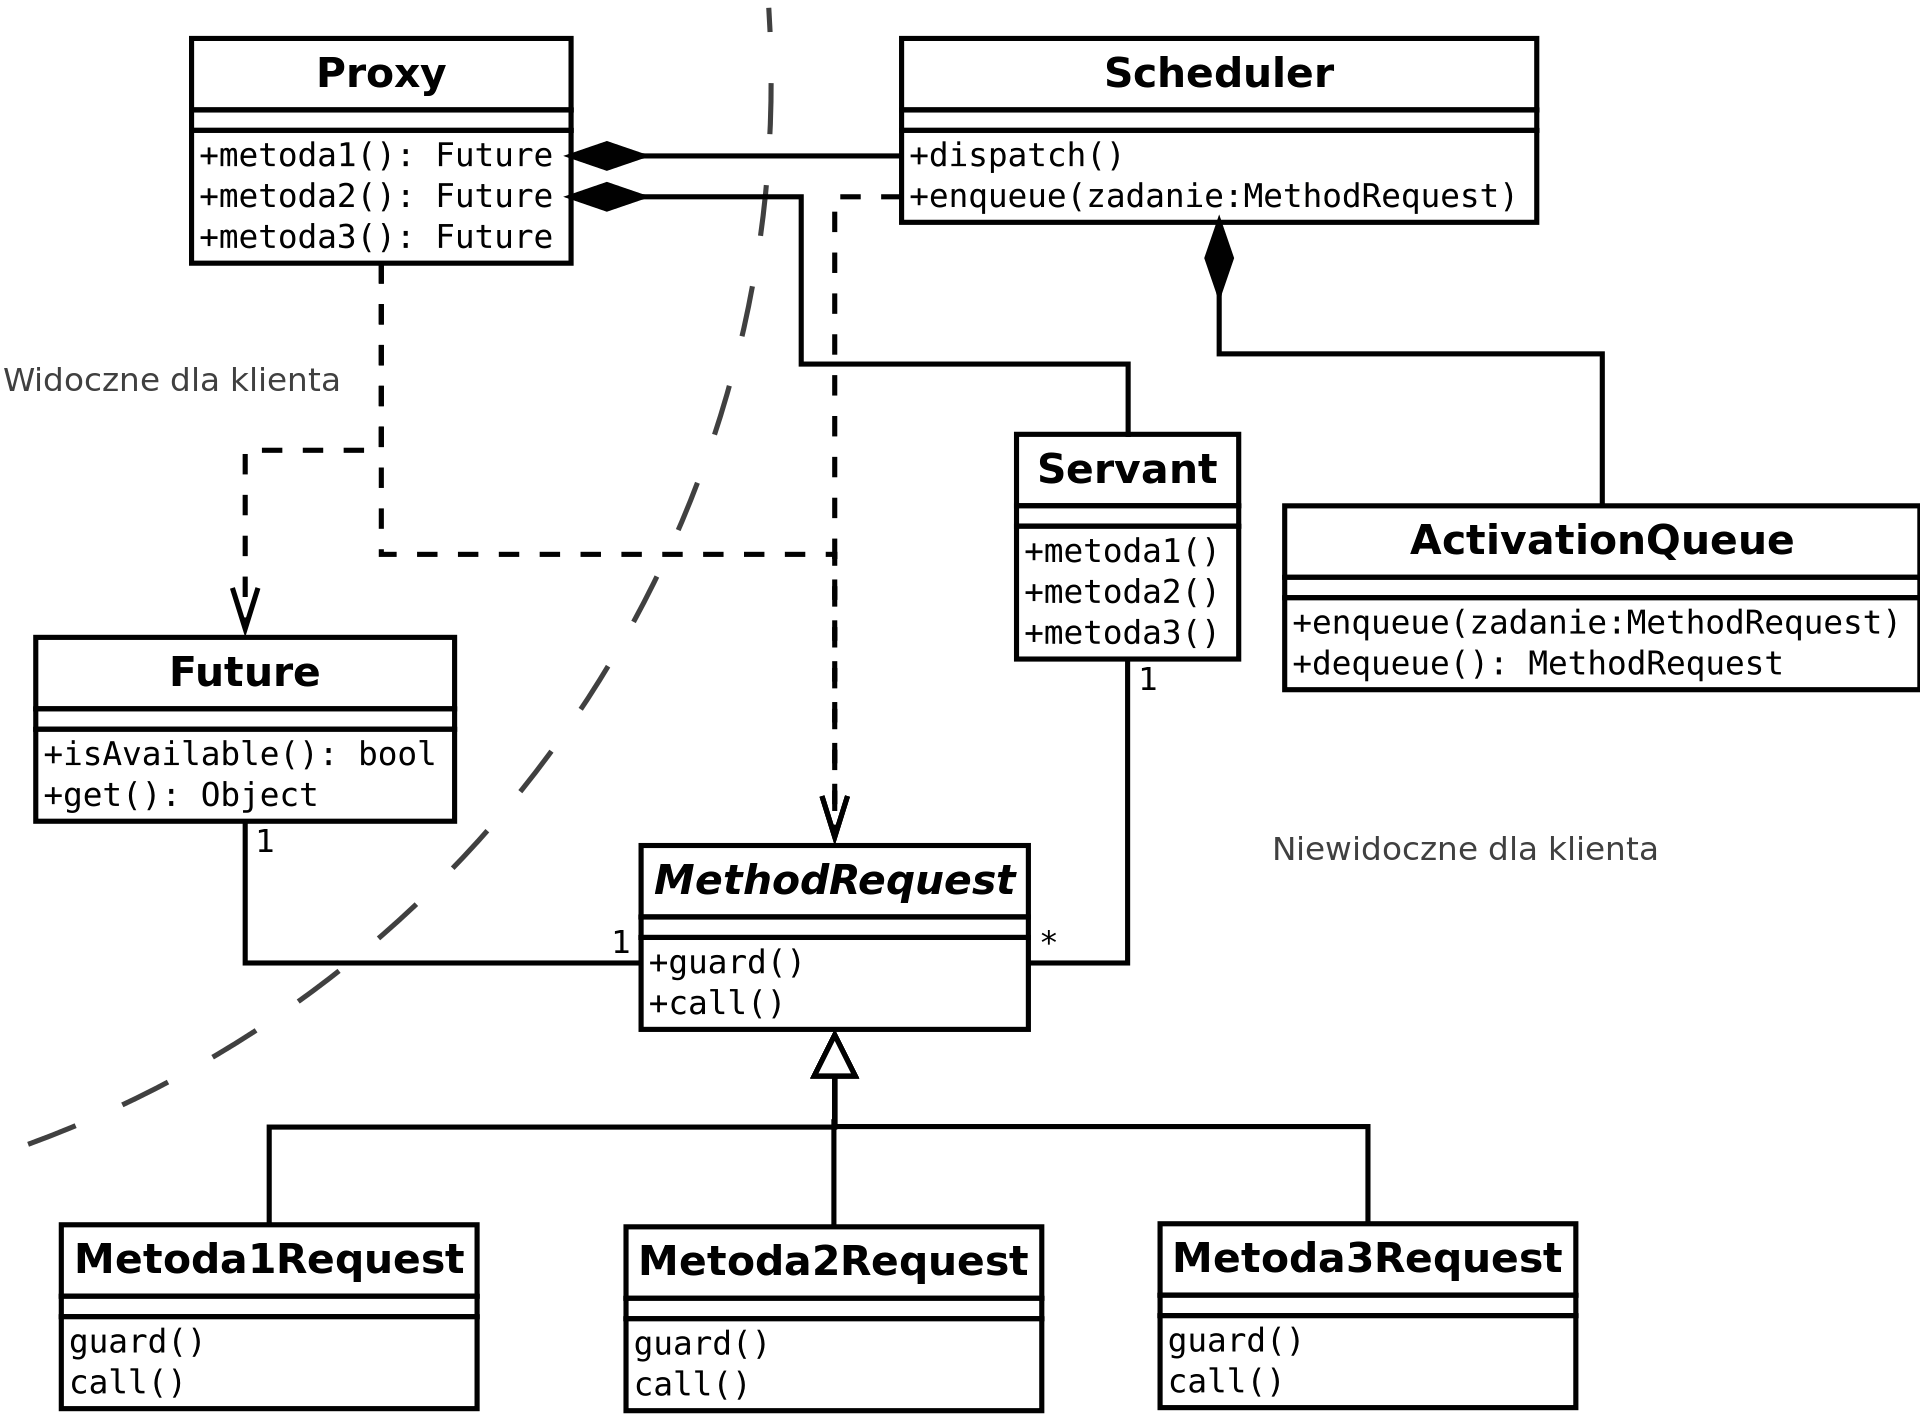
\includegraphics{image.png}
\caption{image.png}
\end{figure}

\[ \text{Diagram UML wzorca Active object} \]

    W trakcie wykonania tego laboratorium powstała następująca struktura:

\begin{verbatim}
tw-lab7/src/main/java/pl/edu/agh/tw/knapp/lab7
    activeobject
        buffer
            Buffer.java
            BufferProxy.java
        MethodRequest.java
        MethodRequestQueue.java
        Scheduler.java
        SimpleFuture.java
    demo
        Consumer.java
        Logger.java
        Main.java
        Producer.java
        RandomSleeper.java
        Worker.java
\end{verbatim}

Pakiet \texttt{activeobject} zawiera implementację współbieżnego wzorcu
projectowego \emph{Active Object}, w tym czasie \texttt{demo} zawiera
przykładową implementację korzystającą z tego wzorca (problem
producenta-konsumenta).

    \hypertarget{active-object}{%
\subsection{Active Object}\label{active-object}}

Jak już zostało wspomniane wcześniej, wzorzec \emph{Active Object}
składa się z sześciu elementów. Pakiet \texttt{activeobject} zawiera
właśnie 6 klas, reprezentujących poszczególne elementy tego wzorca.

    \hypertarget{buffert}{%
\subsubsection{\texorpdfstring{\texttt{Buffer\textless{}T\textgreater{}}}{Buffer\textless T\textgreater{}}}\label{buffert}}

Jest to klasa, reprezentująca bufor. Zawiera samą funkcjonalność, bez
logiki związanej z synchronizacją. We wzorcu \emph{Active Object} tej
klasie odpowiada \textbf{Servant}, jest to bowiem obiekt, do którego
chcemy zapewnić współbieżny dostęp.

Implementacja wygląda następująco:

\begin{Shaded}
\begin{Highlighting}[]
\CommentTok{// Buffer.java}

\KeywordTok{package}\ImportTok{ pl}\OperatorTok{.}\ImportTok{edu}\OperatorTok{.}\ImportTok{agh}\OperatorTok{.}\ImportTok{tw}\OperatorTok{.}\ImportTok{knapp}\OperatorTok{.}\ImportTok{lab7}\OperatorTok{.}\ImportTok{activeobject}\OperatorTok{.}\ImportTok{buffer}\OperatorTok{;}

\KeywordTok{import} \ImportTok{java}\OperatorTok{.}\ImportTok{util}\OperatorTok{.}\ImportTok{ArrayList}\OperatorTok{;}
\KeywordTok{import} \ImportTok{java}\OperatorTok{.}\ImportTok{util}\OperatorTok{.}\ImportTok{Collections}\OperatorTok{;}
\KeywordTok{import} \ImportTok{java}\OperatorTok{.}\ImportTok{util}\OperatorTok{.}\ImportTok{List}\OperatorTok{;}

\KeywordTok{public} \KeywordTok{class} \BuiltInTok{Buffer}\OperatorTok{\textless{}}\NormalTok{T}\OperatorTok{\textgreater{}} \OperatorTok{\{}
    \KeywordTok{private} \DataTypeTok{final} \BuiltInTok{List}\OperatorTok{\textless{}}\NormalTok{T}\OperatorTok{\textgreater{}}\NormalTok{ buffer}\OperatorTok{;}
    \KeywordTok{private} \DataTypeTok{int}\NormalTok{ bufferPos }\OperatorTok{=} \DecValTok{0}\OperatorTok{;}
    \KeywordTok{private} \DataTypeTok{int}\NormalTok{ bufferActualSize }\OperatorTok{=} \DecValTok{0}\OperatorTok{;}

    \KeywordTok{public} \BuiltInTok{Buffer}\OperatorTok{(}\DataTypeTok{int}\NormalTok{ capacity}\OperatorTok{)} \OperatorTok{\{}
\NormalTok{        buffer }\OperatorTok{=} \KeywordTok{new} \BuiltInTok{ArrayList}\OperatorTok{\textless{}\textgreater{}(}\BuiltInTok{Collections}\OperatorTok{.}\FunctionTok{nCopies}\OperatorTok{(}\NormalTok{capacity}\OperatorTok{,} \KeywordTok{null}\OperatorTok{));}
    \OperatorTok{\}}

    \KeywordTok{public} \DataTypeTok{boolean} \FunctionTok{put}\OperatorTok{(}\NormalTok{T element}\OperatorTok{)} \OperatorTok{\{}
        \ControlFlowTok{if} \OperatorTok{(}\FunctionTok{isFull}\OperatorTok{())}
            \ControlFlowTok{return} \KeywordTok{false}\OperatorTok{;}

        \DataTypeTok{var}\NormalTok{ index }\OperatorTok{=} \OperatorTok{(}\NormalTok{bufferPos }\OperatorTok{+}\NormalTok{ bufferActualSize}\OperatorTok{)} \OperatorTok{\%}\NormalTok{ buffer}\OperatorTok{.}\FunctionTok{size}\OperatorTok{();}
        \OperatorTok{++}\NormalTok{bufferActualSize}\OperatorTok{;}
\NormalTok{        buffer}\OperatorTok{.}\FunctionTok{set}\OperatorTok{(}\NormalTok{index}\OperatorTok{,}\NormalTok{ element}\OperatorTok{);}

        \ControlFlowTok{return} \KeywordTok{true}\OperatorTok{;}
    \OperatorTok{\}}

    \KeywordTok{public}\NormalTok{ T }\FunctionTok{pop}\OperatorTok{()} \OperatorTok{\{}
        \ControlFlowTok{if} \OperatorTok{(}\FunctionTok{isEmpty}\OperatorTok{())}
            \ControlFlowTok{return} \KeywordTok{null}\OperatorTok{;}

        \DataTypeTok{var}\NormalTok{ result }\OperatorTok{=}\NormalTok{ buffer}\OperatorTok{.}\FunctionTok{get}\OperatorTok{(}\NormalTok{bufferPos}\OperatorTok{);}
\NormalTok{        bufferPos }\OperatorTok{=} \OperatorTok{(}\NormalTok{bufferPos }\OperatorTok{+} \DecValTok{1}\OperatorTok{)} \OperatorTok{\%}\NormalTok{ buffer}\OperatorTok{.}\FunctionTok{size}\OperatorTok{();}
        \OperatorTok{{-}{-}}\NormalTok{bufferActualSize}\OperatorTok{;}

        \ControlFlowTok{return}\NormalTok{ result}\OperatorTok{;}
    \OperatorTok{\}}

    \KeywordTok{public} \DataTypeTok{int} \FunctionTok{size}\OperatorTok{()} \OperatorTok{\{}
        \ControlFlowTok{return}\NormalTok{ bufferActualSize}\OperatorTok{;}
    \OperatorTok{\}}

    \KeywordTok{public} \DataTypeTok{int} \FunctionTok{capacity}\OperatorTok{()} \OperatorTok{\{}
        \ControlFlowTok{return}\NormalTok{ buffer}\OperatorTok{.}\FunctionTok{size}\OperatorTok{();}
    \OperatorTok{\}}

    \KeywordTok{public} \DataTypeTok{boolean} \FunctionTok{isEmpty}\OperatorTok{()} \OperatorTok{\{}
        \ControlFlowTok{return} \FunctionTok{size}\OperatorTok{()} \OperatorTok{==} \DecValTok{0}\OperatorTok{;}
    \OperatorTok{\}}

    \KeywordTok{public} \DataTypeTok{boolean} \FunctionTok{isNotEmpty}\OperatorTok{()} \OperatorTok{\{}
        \ControlFlowTok{return} \OperatorTok{!}\FunctionTok{isEmpty}\OperatorTok{();}
    \OperatorTok{\}}

    \KeywordTok{public} \DataTypeTok{boolean} \FunctionTok{isFull}\OperatorTok{()} \OperatorTok{\{}
        \ControlFlowTok{return} \FunctionTok{size}\OperatorTok{()} \OperatorTok{==} \FunctionTok{capacity}\OperatorTok{();}
    \OperatorTok{\}}

    \KeywordTok{public} \DataTypeTok{boolean} \FunctionTok{isNotFull}\OperatorTok{()} \OperatorTok{\{}
        \ControlFlowTok{return} \OperatorTok{!}\FunctionTok{isFull}\OperatorTok{();}
    \OperatorTok{\}}
\OperatorTok{\}}
\end{Highlighting}
\end{Shaded}

Jak wynika z implementacji, jest to bufor cykliczny typu FIFO.

    \hypertarget{bufferproxyt}{%
\subsubsection{\texorpdfstring{\texttt{BufferProxy\textless{}T\textgreater{}}}{BufferProxy\textless T\textgreater{}}}\label{bufferproxyt}}

Klasa posiadająca metody o tych samych nazwach i argumentach co i
\texttt{Buffer}, lecz zwracających
\texttt{Future\textless{}T\textgreater{}} zamiast \texttt{T} (gdzie
\texttt{T} - typ zwracany przez oryginalne metody klasy
\texttt{Buffer}). Generuje odpowiednie żądania w imieniu wywołującego
wątku. Jak już wynika z samej nazwy, we wzorcu \emph{Active Object}
odpowiednikiem jest \textbf{Proxy}.

Implementacja tej klasy jest następująca:

\begin{Shaded}
\begin{Highlighting}[]
\CommentTok{// BufferProxy.java}

\KeywordTok{package}\ImportTok{ pl}\OperatorTok{.}\ImportTok{edu}\OperatorTok{.}\ImportTok{agh}\OperatorTok{.}\ImportTok{tw}\OperatorTok{.}\ImportTok{knapp}\OperatorTok{.}\ImportTok{lab7}\OperatorTok{.}\ImportTok{activeobject}\OperatorTok{.}\ImportTok{buffer}\OperatorTok{;}

\KeywordTok{import} \ImportTok{pl}\OperatorTok{.}\ImportTok{edu}\OperatorTok{.}\ImportTok{agh}\OperatorTok{.}\ImportTok{tw}\OperatorTok{.}\ImportTok{knapp}\OperatorTok{.}\ImportTok{lab7}\OperatorTok{.}\ImportTok{activeobject}\OperatorTok{.}\ImportTok{MethodRequest}\OperatorTok{;}
\KeywordTok{import} \ImportTok{pl}\OperatorTok{.}\ImportTok{edu}\OperatorTok{.}\ImportTok{agh}\OperatorTok{.}\ImportTok{tw}\OperatorTok{.}\ImportTok{knapp}\OperatorTok{.}\ImportTok{lab7}\OperatorTok{.}\ImportTok{activeobject}\OperatorTok{.}\ImportTok{Scheduler}\OperatorTok{;}

\KeywordTok{import} \ImportTok{java}\OperatorTok{.}\ImportTok{util}\OperatorTok{.}\ImportTok{concurrent}\OperatorTok{.}\ImportTok{Future}\OperatorTok{;}
\KeywordTok{import} \ImportTok{java}\OperatorTok{.}\ImportTok{util}\OperatorTok{.}\ImportTok{function}\OperatorTok{.}\ImportTok{Supplier}\OperatorTok{;}

\KeywordTok{public} \KeywordTok{class}\NormalTok{ BufferProxy}\OperatorTok{\textless{}}\NormalTok{T}\OperatorTok{\textgreater{}} \OperatorTok{\{}
    \KeywordTok{private} \DataTypeTok{final} \BuiltInTok{Buffer}\OperatorTok{\textless{}}\NormalTok{T}\OperatorTok{\textgreater{}}\NormalTok{ buffer}\OperatorTok{;}
    \KeywordTok{private} \DataTypeTok{final}\NormalTok{ Scheduler scheduler}\OperatorTok{;}

    \KeywordTok{public} \FunctionTok{BufferProxy}\OperatorTok{(}\DataTypeTok{int}\NormalTok{ capacity}\OperatorTok{,}\NormalTok{ Scheduler scheduler}\OperatorTok{)} \OperatorTok{\{}
\NormalTok{        buffer }\OperatorTok{=} \KeywordTok{new} \BuiltInTok{Buffer}\OperatorTok{\textless{}\textgreater{}(}\NormalTok{capacity}\OperatorTok{);}
        \KeywordTok{this}\OperatorTok{.}\FunctionTok{scheduler} \OperatorTok{=}\NormalTok{ scheduler}\OperatorTok{;}
    \OperatorTok{\}}

    \KeywordTok{public} \BuiltInTok{Future}\OperatorTok{\textless{}}\BuiltInTok{Boolean}\OperatorTok{\textgreater{}} \FunctionTok{put}\OperatorTok{(}\NormalTok{T element}\OperatorTok{)} \OperatorTok{\{}
        \ControlFlowTok{return}\NormalTok{ scheduler}\OperatorTok{.}\FunctionTok{enqueue}\OperatorTok{(}\FunctionTok{mkMethodRequest}\OperatorTok{(()} \OperatorTok{{-}\textgreater{}}
\NormalTok{            buffer}\OperatorTok{.}\FunctionTok{put}\OperatorTok{(}\NormalTok{element}\OperatorTok{),}\NormalTok{ buffer}\OperatorTok{::}\NormalTok{isNotFull}\OperatorTok{));}
    \OperatorTok{\}}

    \KeywordTok{public} \BuiltInTok{Future}\OperatorTok{\textless{}}\NormalTok{T}\OperatorTok{\textgreater{}} \FunctionTok{pop}\OperatorTok{()} \OperatorTok{\{}
        \ControlFlowTok{return}\NormalTok{ scheduler}\OperatorTok{.}\FunctionTok{enqueue}\OperatorTok{(}\FunctionTok{mkMethodRequest}\OperatorTok{(}\NormalTok{buffer}\OperatorTok{::}\NormalTok{pop}\OperatorTok{,}\NormalTok{ buffer}\OperatorTok{::}\NormalTok{isNotEmpty}\OperatorTok{));}
    \OperatorTok{\}}

    \KeywordTok{public} \BuiltInTok{Future}\OperatorTok{\textless{}}\BuiltInTok{Integer}\OperatorTok{\textgreater{}} \FunctionTok{size}\OperatorTok{()} \OperatorTok{\{}
        \ControlFlowTok{return}\NormalTok{ scheduler}\OperatorTok{.}\FunctionTok{enqueue}\OperatorTok{(}\FunctionTok{mkMethodRequest}\OperatorTok{(}\NormalTok{buffer}\OperatorTok{::}\NormalTok{size}\OperatorTok{,} \OperatorTok{()} \OperatorTok{{-}\textgreater{}} \KeywordTok{true}\OperatorTok{));}
    \OperatorTok{\}}

    \KeywordTok{public} \BuiltInTok{Future}\OperatorTok{\textless{}}\BuiltInTok{Integer}\OperatorTok{\textgreater{}} \FunctionTok{capacity}\OperatorTok{()} \OperatorTok{\{}
        \ControlFlowTok{return}\NormalTok{ scheduler}\OperatorTok{.}\FunctionTok{enqueue}\OperatorTok{(}\FunctionTok{mkMethodRequest}\OperatorTok{(}\NormalTok{buffer}\OperatorTok{::}\NormalTok{capacity}\OperatorTok{,} \OperatorTok{()} \OperatorTok{{-}\textgreater{}} \KeywordTok{true}\OperatorTok{));}
    \OperatorTok{\}}

    \KeywordTok{public} \BuiltInTok{Future}\OperatorTok{\textless{}}\BuiltInTok{Boolean}\OperatorTok{\textgreater{}} \FunctionTok{isEmpty}\OperatorTok{()} \OperatorTok{\{}
        \ControlFlowTok{return}\NormalTok{ scheduler}\OperatorTok{.}\FunctionTok{enqueue}\OperatorTok{(}\FunctionTok{mkMethodRequest}\OperatorTok{(}\NormalTok{buffer}\OperatorTok{::}\NormalTok{isEmpty}\OperatorTok{,} \OperatorTok{()} \OperatorTok{{-}\textgreater{}} \KeywordTok{true}\OperatorTok{));}
    \OperatorTok{\}}

    \KeywordTok{public} \BuiltInTok{Future}\OperatorTok{\textless{}}\BuiltInTok{Boolean}\OperatorTok{\textgreater{}} \FunctionTok{isNotEmpty}\OperatorTok{()} \OperatorTok{\{}
        \ControlFlowTok{return}\NormalTok{ scheduler}\OperatorTok{.}\FunctionTok{enqueue}\OperatorTok{(}\FunctionTok{mkMethodRequest}\OperatorTok{(}\NormalTok{buffer}\OperatorTok{::}\NormalTok{isNotEmpty}\OperatorTok{,} \OperatorTok{()} \OperatorTok{{-}\textgreater{}} \KeywordTok{true}\OperatorTok{));}
    \OperatorTok{\}}

    \KeywordTok{public} \BuiltInTok{Future}\OperatorTok{\textless{}}\BuiltInTok{Boolean}\OperatorTok{\textgreater{}} \FunctionTok{isFull}\OperatorTok{()} \OperatorTok{\{}
        \ControlFlowTok{return}\NormalTok{ scheduler}\OperatorTok{.}\FunctionTok{enqueue}\OperatorTok{(}\FunctionTok{mkMethodRequest}\OperatorTok{(}\NormalTok{buffer}\OperatorTok{::}\NormalTok{isFull}\OperatorTok{,} \OperatorTok{()} \OperatorTok{{-}\textgreater{}} \KeywordTok{true}\OperatorTok{));}
    \OperatorTok{\}}

    \KeywordTok{public} \BuiltInTok{Future}\OperatorTok{\textless{}}\BuiltInTok{Boolean}\OperatorTok{\textgreater{}} \FunctionTok{isNotFull}\OperatorTok{()} \OperatorTok{\{}
        \ControlFlowTok{return}\NormalTok{ scheduler}\OperatorTok{.}\FunctionTok{enqueue}\OperatorTok{(}\FunctionTok{mkMethodRequest}\OperatorTok{(}\NormalTok{buffer}\OperatorTok{::}\NormalTok{isNotFull}\OperatorTok{,} \OperatorTok{()} \OperatorTok{{-}\textgreater{}} \KeywordTok{true}\OperatorTok{));}
    \OperatorTok{\}}

    \KeywordTok{private} \DataTypeTok{static} \OperatorTok{\textless{}}\NormalTok{V}\OperatorTok{\textgreater{}}\NormalTok{ MethodRequest}\OperatorTok{\textless{}}\NormalTok{V}\OperatorTok{\textgreater{}} \FunctionTok{mkMethodRequest}\OperatorTok{(}
\NormalTok{        Supplier}\OperatorTok{\textless{}}\NormalTok{V}\OperatorTok{\textgreater{}}\NormalTok{ call}\OperatorTok{,}
\NormalTok{        Supplier}\OperatorTok{\textless{}}\BuiltInTok{Boolean}\OperatorTok{\textgreater{}}\NormalTok{ guard}
    \OperatorTok{)} \OperatorTok{\{}
        \ControlFlowTok{return} \KeywordTok{new}\NormalTok{ MethodRequest}\OperatorTok{\textless{}\textgreater{}()} \OperatorTok{\{}
            \AttributeTok{@Override}
            \KeywordTok{public}\NormalTok{ V }\FunctionTok{call}\OperatorTok{()} \OperatorTok{\{}
                \ControlFlowTok{return}\NormalTok{ call}\OperatorTok{.}\FunctionTok{get}\OperatorTok{();}
            \OperatorTok{\}}

            \AttributeTok{@Override}
            \KeywordTok{public} \DataTypeTok{boolean} \FunctionTok{guard}\OperatorTok{()} \OperatorTok{\{}
                \ControlFlowTok{return}\NormalTok{ guard}\OperatorTok{.}\FunctionTok{get}\OperatorTok{();}
            \OperatorTok{\}}
        \OperatorTok{\};}
    \OperatorTok{\}}
\OperatorTok{\}}
\end{Highlighting}
\end{Shaded}

W celu podniesienia czytelności została utworzona metoda pomocnicza
\texttt{mkMethodRequest}, przyjmująca jako argumenty interfejs
\texttt{call} typu \texttt{Supplier\textless{}V\textgreater{}}, gdzie
\texttt{V} - dowolny typ, oraz interfejs \texttt{guard} typu
\texttt{Supplier\textless{}Boolean\textgreater{}} zwracający
\texttt{true} jeżeli wszystkie warunki zostały spełnione i \texttt{call}
może zostać wywołany, \texttt{false} w przeciwnym przypadku. Metoda ta
zwraca \texttt{MethodRequest\textless{}V\textgreater{}}.

Innymi słowy,

\begin{Shaded}
\begin{Highlighting}[]
\FunctionTok{mkMethodRequest}\OperatorTok{(}\NormalTok{AKCJA}\OperatorTok{,}\NormalTok{ WARUNEK}\OperatorTok{)}
\end{Highlighting}
\end{Shaded}

    \hypertarget{methodrequestt}{%
\subsubsection{\texorpdfstring{\texttt{MethodRequest\textless{}T\textgreater{}}}{MethodRequest\textless T\textgreater{}}}\label{methodrequestt}}

Ten interfejs jest używany do przekazania kontekstu wywołania metody z
\texttt{Proxy} do \texttt{Scheduler}a uruchomionego w osobnym wątku.
Definiuje interfejs dla wykonywania metod Aktywnego Obiektu. Oprócz
metody \texttt{call}, interfejs ten zawiera również metodę
\texttt{guard}, służącą do sprawdzenia, czy warunki związane z
synchronizacją są spełnione. Jak sama nazwa wskazuje, we wzorcu
\emph{Active Object} odpowiednikiem jest \textbf{MethodRequest}.

Implementacja:

\begin{Shaded}
\begin{Highlighting}[]
\CommentTok{// MethodRequest.java}

\KeywordTok{package}\ImportTok{ pl}\OperatorTok{.}\ImportTok{edu}\OperatorTok{.}\ImportTok{agh}\OperatorTok{.}\ImportTok{tw}\OperatorTok{.}\ImportTok{knapp}\OperatorTok{.}\ImportTok{lab7}\OperatorTok{.}\ImportTok{activeobject}\OperatorTok{;}

\KeywordTok{public} \KeywordTok{interface}\NormalTok{ MethodRequest}\OperatorTok{\textless{}}\NormalTok{T}\OperatorTok{\textgreater{}} \OperatorTok{\{}
\NormalTok{    T }\FunctionTok{call}\OperatorTok{();}
    \DataTypeTok{boolean} \FunctionTok{guard}\OperatorTok{();}
\OperatorTok{\}}
\end{Highlighting}
\end{Shaded}

    \hypertarget{methodrequestqueuet-extends-methodrequest}{%
\subsubsection{\texorpdfstring{\texttt{MethodRequestQueue\textless{}T\ extends\ MethodRequest\textless{}?\textgreater{}\textgreater{}}}{MethodRequestQueue\textless T extends MethodRequest\textless?\textgreater\textgreater{}}}\label{methodrequestqueuet-extends-methodrequest}}

Zawiera bufor oczekujących \texttt{MethodRequest} utworzonych przez
\texttt{Proxy}. Jest zasobem dzielonym dla wątków klienta i pracownika
(\texttt{Servant}) - pierwszy jest producentem żądań metody, drugi ich
konsumentem (przez \texttt{Scheduler}). We wzorcu \emph{Active Object}
odpowiednikiem jest \textbf{ActivationQueue}.

\hypertarget{dostux119pne-metody}{%
\paragraph{Dostępne metody}\label{dostux119pne-metody}}

\begin{itemize}
\tightlist
\item
  \texttt{void\ put(T\ element)} - umieszcza element w kolejce
\item
  \texttt{void\ forEachReady(Consumer\textless{}?\ super\ T\textgreater{}\ consumer)}
  - \texttt{consumer} zostanie wywołany dla elementów ze spełnionymi
  warunkami synchronizacji (inaczej mówiąc, dla tych obiektów dla
  których metoda \texttt{guard} zwróciła \texttt{true})
\item
  \texttt{int\ currentSize()} - rozmiar aktywnej kolejki
\item
  \texttt{int\ waitSize()} - rozmiar kolejki oczekiwania
\item
  \texttt{int\ size()} - łączny rozmiar w/w kolejek
\end{itemize}

\hypertarget{problem-naiwnej-implementacji}{%
\paragraph{Problem naiwnej
implementacji}\label{problem-naiwnej-implementacji}}

W przypadku \emph{naiwnej} implementacji, można w łatwy sposób dojść do
zagłodzenia niektórych \texttt{MethodRequest}. Wystarczy, że mamy bufor
o rozmiarze \texttt{1}, do kolejki \texttt{MethodRequestQueue} kolejno
dodajemy:

\begin{verbatim}
<put(0)>  # dodaje 0
<put(1)>  # dodanie się nie powiodło: kolejka jest pełna
<pop>     # usuwa 0
<put(2)>  # dodaje 2
\end{verbatim}

Po wywołaniu \texttt{forEachReady} w kolejce zostanie
\texttt{\textless{}put(1)\textgreater{}}. Jeżeli będziemy wykonywać
kolejne

\begin{verbatim}
<pop>     # usuwa 2
<put(n)>  # dodaje n
\end{verbatim}

to \texttt{\textless{}put(1)\textgreater{}} nigdy nie zostanie wykonane.

W celu rozwiązania tego problemu, \textbf{zostały utworzone 2 osobne
kolejki}: \texttt{currentQueue} oraz \texttt{waitQueue}.

\begin{itemize}
\tightlist
\item
  \texttt{currentQueue} zawiera te \texttt{MethodRequest}, które trzeba
  spróbować wykonac przy kolejnym wywołaniu \texttt{forEachReady}
\item
  \texttt{waitQueue} zawiera te \texttt{MethodRequest}, warunki
  synchronizacji których nie zostały spełnione podczas wywołania
  \texttt{forEachReady}
\end{itemize}

\hypertarget{algorytm}{%
\paragraph{Algorytm}\label{algorytm}}

\begin{enumerate}
\def\labelenumi{\arabic{enumi}.}
\tightlist
\item
  Dopóki kolejka \texttt{currentQueue} nie jest pusta:

  \begin{enumerate}
  \def\labelenumii{\arabic{enumii}.}
  \tightlist
  \item
    Ściągnij element z \texttt{currentQueue}
  \item
    Jeżeli warunki synchronizacji zostały spełnione, wywołaj
    \texttt{consumer.accept(element)}

    \begin{itemize}
    \tightlist
    \item
      Sprawdź, czy dla którychś elementów z \texttt{waitQueue} nie
      zostały spełnione warunki synchronizacji. Jeżeli tak, wywołaj
      \texttt{Consumer::accept} dla tych elementów i usuń z kolejki
      \texttt{waitQueue}
    \end{itemize}
  \item
    W przeciwnym przypadku dodaj do \texttt{waitQueue}
  \end{enumerate}
\item
  Wykonaj \texttt{swap(currentQueue,\ waitQueue)}
\end{enumerate}

    \hypertarget{implementacja}{%
\paragraph{Implementacja}\label{implementacja}}

\begin{Shaded}
\begin{Highlighting}[]
\CommentTok{// MethodRequestQueue.java}

\KeywordTok{package}\ImportTok{ pl}\OperatorTok{.}\ImportTok{edu}\OperatorTok{.}\ImportTok{agh}\OperatorTok{.}\ImportTok{tw}\OperatorTok{.}\ImportTok{knapp}\OperatorTok{.}\ImportTok{lab7}\OperatorTok{.}\ImportTok{activeobject}\OperatorTok{;}

\KeywordTok{import} \ImportTok{java}\OperatorTok{.}\ImportTok{util}\OperatorTok{.}\ImportTok{ArrayDeque}\OperatorTok{;}
\KeywordTok{import} \ImportTok{java}\OperatorTok{.}\ImportTok{util}\OperatorTok{.}\ImportTok{Queue}\OperatorTok{;}
\KeywordTok{import} \ImportTok{java}\OperatorTok{.}\ImportTok{util}\OperatorTok{.}\ImportTok{function}\OperatorTok{.}\ImportTok{Consumer}\OperatorTok{;}

\KeywordTok{public} \KeywordTok{class}\NormalTok{ MethodRequestQueue}\OperatorTok{\textless{}}\NormalTok{T }\KeywordTok{extends}\NormalTok{ MethodRequest}\OperatorTok{\textless{}?\textgreater{}\textgreater{}} \OperatorTok{\{}
    \KeywordTok{private} \BuiltInTok{Queue}\OperatorTok{\textless{}}\NormalTok{T}\OperatorTok{\textgreater{}}\NormalTok{ waitQueue }\OperatorTok{=} \KeywordTok{new} \BuiltInTok{ArrayDeque}\OperatorTok{\textless{}\textgreater{}();}
    \KeywordTok{private} \BuiltInTok{Queue}\OperatorTok{\textless{}}\NormalTok{T}\OperatorTok{\textgreater{}}\NormalTok{ currentQueue }\OperatorTok{=} \KeywordTok{new} \BuiltInTok{ArrayDeque}\OperatorTok{\textless{}\textgreater{}();}

    \KeywordTok{public} \DataTypeTok{void} \FunctionTok{put}\OperatorTok{(}\NormalTok{T element}\OperatorTok{)} \OperatorTok{\{}
\NormalTok{        currentQueue}\OperatorTok{.}\FunctionTok{add}\OperatorTok{(}\NormalTok{element}\OperatorTok{);}
    \OperatorTok{\}}

    \KeywordTok{public} \DataTypeTok{void} \FunctionTok{forEachReady}\OperatorTok{(}\NormalTok{Consumer}\OperatorTok{\textless{}?} \KeywordTok{super}\NormalTok{ T}\OperatorTok{\textgreater{}}\NormalTok{ consumer}\OperatorTok{)} \OperatorTok{\{}
        \ControlFlowTok{while} \OperatorTok{(!}\NormalTok{currentQueue}\OperatorTok{.}\FunctionTok{isEmpty}\OperatorTok{())} \OperatorTok{\{}
            \DataTypeTok{var}\NormalTok{ element }\OperatorTok{=}\NormalTok{ currentQueue}\OperatorTok{.}\FunctionTok{poll}\OperatorTok{();}

            \ControlFlowTok{if} \OperatorTok{(}\NormalTok{element}\OperatorTok{.}\FunctionTok{guard}\OperatorTok{())} \OperatorTok{\{}
\NormalTok{                consumer}\OperatorTok{.}\FunctionTok{accept}\OperatorTok{(}\NormalTok{element}\OperatorTok{);}

                \CommentTok{// try to execute something from the wait queue}
                \ControlFlowTok{for} \OperatorTok{(}\DataTypeTok{int}\NormalTok{ i }\OperatorTok{=} \DecValTok{0}\OperatorTok{;}\NormalTok{ i }\OperatorTok{\textless{}}\NormalTok{ waitQueue}\OperatorTok{.}\FunctionTok{size}\OperatorTok{();}\NormalTok{ i}\OperatorTok{++)} \OperatorTok{\{}
                    \DataTypeTok{var}\NormalTok{ waiting }\OperatorTok{=}\NormalTok{ waitQueue}\OperatorTok{.}\FunctionTok{poll}\OperatorTok{();}

                    \ControlFlowTok{if} \OperatorTok{(}\NormalTok{waiting}\OperatorTok{.}\FunctionTok{guard}\OperatorTok{())} \OperatorTok{\{}
\NormalTok{                        consumer}\OperatorTok{.}\FunctionTok{accept}\OperatorTok{(}\NormalTok{waiting}\OperatorTok{);}
                    \OperatorTok{\}} \ControlFlowTok{else} \OperatorTok{\{}
\NormalTok{                        waitQueue}\OperatorTok{.}\FunctionTok{add}\OperatorTok{(}\NormalTok{waiting}\OperatorTok{);}
                    \OperatorTok{\}}
                \OperatorTok{\}}
            \OperatorTok{\}} \ControlFlowTok{else} \OperatorTok{\{}
\NormalTok{                waitQueue}\OperatorTok{.}\FunctionTok{add}\OperatorTok{(}\NormalTok{element}\OperatorTok{);}
            \OperatorTok{\}}
        \OperatorTok{\}}

        \CommentTok{// swap, currentQueue is empty now,}
        \CommentTok{// waitQueue may be not empty}
        \DataTypeTok{var}\NormalTok{ tmp }\OperatorTok{=}\NormalTok{ waitQueue}\OperatorTok{;}
\NormalTok{        waitQueue }\OperatorTok{=}\NormalTok{ currentQueue}\OperatorTok{;}
\NormalTok{        currentQueue }\OperatorTok{=}\NormalTok{ tmp}\OperatorTok{;}
    \OperatorTok{\}}

    \KeywordTok{public} \DataTypeTok{int} \FunctionTok{currentSize}\OperatorTok{()} \OperatorTok{\{}
        \ControlFlowTok{return}\NormalTok{ currentQueue}\OperatorTok{.}\FunctionTok{size}\OperatorTok{();}
    \OperatorTok{\}}

    \KeywordTok{public} \DataTypeTok{int} \FunctionTok{waitSize}\OperatorTok{()} \OperatorTok{\{}
        \ControlFlowTok{return}\NormalTok{ waitQueue}\OperatorTok{.}\FunctionTok{size}\OperatorTok{();}
    \OperatorTok{\}}

    \KeywordTok{public} \DataTypeTok{int} \FunctionTok{size}\OperatorTok{()} \OperatorTok{\{}
        \ControlFlowTok{return} \FunctionTok{currentSize}\OperatorTok{()} \OperatorTok{+} \FunctionTok{waitSize}\OperatorTok{();}
    \OperatorTok{\}}
\OperatorTok{\}}
\end{Highlighting}
\end{Shaded}

    \hypertarget{scheduler}{%
\subsubsection{\texorpdfstring{\texttt{Scheduler}}{Scheduler}}\label{scheduler}}

Wykonuje się w osobnym wątku, zarządzając \texttt{MethodRequestQueue}.
Zawiera odwzorowanie między
\texttt{MethodRequest\textless{}?\textgreater{}} a
\texttt{Future\textless{}?\textgreater{}}. Jak sama nazwa wskazuje, we
wzorcu \emph{Active Object} odpowiednikiem jest \textbf{Scheduler}.

Podczas wykonania metody
\texttt{\textless{}T\textgreater{}\ Future\textless{}T\textgreater{}\ enqueue(MethodRequest\textless{}T\textgreater{}\ methodRequest)}
odwzorowanie między \texttt{MethodRequest\textless{}?\textgreater{}} a
\texttt{Future\textless{}?\textgreater{}} zostaje aktualizowane:
zapamiętujemy, dla którego \texttt{MethodRequest} został stworzony który
\texttt{Future}, aby później moć przekazać wynik pochodzący z
\texttt{MethodRequest} do odpowiedniego \texttt{Future}.

Implementacja wygląda następująco:

\begin{Shaded}
\begin{Highlighting}[]
\CommentTok{// Scheduler.java}

\KeywordTok{package}\ImportTok{ pl}\OperatorTok{.}\ImportTok{edu}\OperatorTok{.}\ImportTok{agh}\OperatorTok{.}\ImportTok{tw}\OperatorTok{.}\ImportTok{knapp}\OperatorTok{.}\ImportTok{lab7}\OperatorTok{.}\ImportTok{activeobject}\OperatorTok{;}

\KeywordTok{import} \ImportTok{java}\OperatorTok{.}\ImportTok{util}\OperatorTok{.}\ImportTok{HashMap}\OperatorTok{;}
\KeywordTok{import} \ImportTok{java}\OperatorTok{.}\ImportTok{util}\OperatorTok{.}\ImportTok{Map}\OperatorTok{;}
\KeywordTok{import} \ImportTok{java}\OperatorTok{.}\ImportTok{util}\OperatorTok{.}\ImportTok{concurrent}\OperatorTok{.}\ImportTok{Future}\OperatorTok{;}

\KeywordTok{public} \KeywordTok{class}\NormalTok{ Scheduler }\KeywordTok{extends} \BuiltInTok{Thread} \OperatorTok{\{}
    \KeywordTok{private} \DataTypeTok{final}\NormalTok{ MethodRequestQueue}\OperatorTok{\textless{}}\NormalTok{MethodRequest}\OperatorTok{\textless{}?\textgreater{}\textgreater{}}\NormalTok{ methodRequestQueue }\OperatorTok{=}
        \KeywordTok{new}\NormalTok{ MethodRequestQueue}\OperatorTok{\textless{}\textgreater{}();}

    \KeywordTok{private} \DataTypeTok{final} \BuiltInTok{Map}\OperatorTok{\textless{}}\NormalTok{MethodRequest}\OperatorTok{\textless{}?\textgreater{},}\NormalTok{ SimpleFuture}\OperatorTok{\textless{}?\textgreater{}\textgreater{}}\NormalTok{ methodRequestFutureMap }\OperatorTok{=}
        \KeywordTok{new} \BuiltInTok{HashMap}\OperatorTok{\textless{}\textgreater{}();}

    \KeywordTok{private} \DataTypeTok{boolean}\NormalTok{ isRunning }\OperatorTok{=} \KeywordTok{true}\OperatorTok{;}

    \KeywordTok{private} \DataTypeTok{int}\NormalTok{ autoDispatchMod }\OperatorTok{=} \DecValTok{5}\OperatorTok{;}

    \KeywordTok{public} \DataTypeTok{void} \FunctionTok{setAutoDispatchMod}\OperatorTok{(}\DataTypeTok{int}\NormalTok{ autoDispatchMod}\OperatorTok{)} \OperatorTok{\{}
        \KeywordTok{this}\OperatorTok{.}\FunctionTok{autoDispatchMod} \OperatorTok{=}\NormalTok{ autoDispatchMod}\OperatorTok{;}
    \OperatorTok{\}}

    \KeywordTok{public} \DataTypeTok{int} \FunctionTok{getAutoDispatchMod}\OperatorTok{()} \OperatorTok{\{}
        \ControlFlowTok{return}\NormalTok{ autoDispatchMod}\OperatorTok{;}
    \OperatorTok{\}}

    \KeywordTok{public} \OperatorTok{\textless{}}\NormalTok{T}\OperatorTok{\textgreater{}} \BuiltInTok{Future}\OperatorTok{\textless{}}\NormalTok{T}\OperatorTok{\textgreater{}} \FunctionTok{enqueue}\OperatorTok{(}\NormalTok{MethodRequest}\OperatorTok{\textless{}}\NormalTok{T}\OperatorTok{\textgreater{}}\NormalTok{ methodRequest}\OperatorTok{)} \OperatorTok{\{}
        \DataTypeTok{var}\NormalTok{ future }\OperatorTok{=} \KeywordTok{new}\NormalTok{ SimpleFuture}\OperatorTok{\textless{}}\NormalTok{T}\OperatorTok{\textgreater{}();}

        \KeywordTok{synchronized} \OperatorTok{(}\KeywordTok{this}\OperatorTok{)} \OperatorTok{\{}
\NormalTok{            methodRequestFutureMap}\OperatorTok{.}\FunctionTok{put}\OperatorTok{(}\NormalTok{methodRequest}\OperatorTok{,}\NormalTok{ future}\OperatorTok{);}
\NormalTok{            methodRequestQueue}\OperatorTok{.}\FunctionTok{put}\OperatorTok{(}\NormalTok{methodRequest}\OperatorTok{);}

            \ControlFlowTok{if} \OperatorTok{(}\NormalTok{methodRequestQueue}\OperatorTok{.}\FunctionTok{size}\OperatorTok{()} \OperatorTok{\%}\NormalTok{ autoDispatchMod }\OperatorTok{==} \DecValTok{0}\OperatorTok{)} \OperatorTok{\{}
                \FunctionTok{dispatch}\OperatorTok{();}
            \OperatorTok{\}}
        \OperatorTok{\}}

        \ControlFlowTok{return}\NormalTok{ future}\OperatorTok{;}
    \OperatorTok{\}}

    \KeywordTok{public} \KeywordTok{synchronized} \DataTypeTok{void} \FunctionTok{dispatch}\OperatorTok{()} \OperatorTok{\{}
        \FunctionTok{notify}\OperatorTok{();}
    \OperatorTok{\}}

    \KeywordTok{public} \KeywordTok{synchronized} \DataTypeTok{void} \FunctionTok{shutdown}\OperatorTok{()} \OperatorTok{\{}
\NormalTok{        isRunning }\OperatorTok{=} \KeywordTok{false}\OperatorTok{;}
        \FunctionTok{notify}\OperatorTok{();}
    \OperatorTok{\}}

    \AttributeTok{@Override}
    \KeywordTok{public} \KeywordTok{synchronized} \DataTypeTok{void} \FunctionTok{run}\OperatorTok{()} \OperatorTok{\{}
        \ControlFlowTok{while} \OperatorTok{(}\NormalTok{isRunning}\OperatorTok{)} \OperatorTok{\{}
            \ControlFlowTok{try} \OperatorTok{\{}
                \FunctionTok{wait}\OperatorTok{();}
            \OperatorTok{\}} \ControlFlowTok{catch} \OperatorTok{(}\BuiltInTok{InterruptedException}\NormalTok{ e}\OperatorTok{)} \OperatorTok{\{}
                \ControlFlowTok{throw} \KeywordTok{new} \BuiltInTok{RuntimeException}\OperatorTok{(}\NormalTok{e}\OperatorTok{);}
            \OperatorTok{\}}

\NormalTok{            methodRequestQueue}\OperatorTok{.}\FunctionTok{forEachReady}\OperatorTok{(}\NormalTok{methodRequest }\OperatorTok{{-}\textgreater{}}
\NormalTok{                methodRequestFutureMap}\OperatorTok{.}\FunctionTok{remove}\OperatorTok{(}\NormalTok{methodRequest}\OperatorTok{).}\FunctionTok{put}\OperatorTok{(}\NormalTok{methodRequest}\OperatorTok{.}\FunctionTok{call}\OperatorTok{()));}
        \OperatorTok{\}}
    \OperatorTok{\}}
\OperatorTok{\}}
\end{Highlighting}
\end{Shaded}

    \hypertarget{simplefuturet}{%
\subsubsection{\texorpdfstring{\texttt{SimpleFuture\textless{}T\textgreater{}}}{SimpleFuture\textless T\textgreater{}}}\label{simplefuturet}}

Implementuje interfejs \texttt{Future\textless{}T\textgreater{}}.
Pozwala klientowi pobranie wyniku wykonania metody, gdy \texttt{Servant}
zakończy jej wykonanie. Po wywołaniu metody w \texttt{Proxy}, obiekt
\texttt{Future} jest od razu zwracany. \texttt{Future} rezerwuje miejsce
na wyniki wywołania metody. Gdy klient chce te wyniki pobrać, albo się
blokuje do czasu pojawienia się wyników, albo periodycznie sprawdza
przez \emph{polling}. We wzorcu \emph{Active Object} odpowiednikiem jest
\textbf{Future}.

Implementacja:

\begin{Shaded}
\begin{Highlighting}[]
\CommentTok{// SimpleFuture.java}

\KeywordTok{package}\ImportTok{ pl}\OperatorTok{.}\ImportTok{edu}\OperatorTok{.}\ImportTok{agh}\OperatorTok{.}\ImportTok{tw}\OperatorTok{.}\ImportTok{knapp}\OperatorTok{.}\ImportTok{lab7}\OperatorTok{.}\ImportTok{activeobject}\OperatorTok{;}

\KeywordTok{import} \ImportTok{org}\OperatorTok{.}\ImportTok{jetbrains}\OperatorTok{.}\ImportTok{annotations}\OperatorTok{.}\ImportTok{NotNull}\OperatorTok{;}

\KeywordTok{import} \ImportTok{java}\OperatorTok{.}\ImportTok{util}\OperatorTok{.}\ImportTok{concurrent}\OperatorTok{.}\ImportTok{CountDownLatch}\OperatorTok{;}
\KeywordTok{import} \ImportTok{java}\OperatorTok{.}\ImportTok{util}\OperatorTok{.}\ImportTok{concurrent}\OperatorTok{.}\ImportTok{Future}\OperatorTok{;}
\KeywordTok{import} \ImportTok{java}\OperatorTok{.}\ImportTok{util}\OperatorTok{.}\ImportTok{concurrent}\OperatorTok{.}\ImportTok{TimeUnit}\OperatorTok{;}
\KeywordTok{import} \ImportTok{java}\OperatorTok{.}\ImportTok{util}\OperatorTok{.}\ImportTok{concurrent}\OperatorTok{.}\ImportTok{TimeoutException}\OperatorTok{;}

\KeywordTok{public} \DataTypeTok{final} \KeywordTok{class}\NormalTok{ SimpleFuture}\OperatorTok{\textless{}}\NormalTok{T}\OperatorTok{\textgreater{}} \KeywordTok{implements} \BuiltInTok{Future}\OperatorTok{\textless{}}\NormalTok{T}\OperatorTok{\textgreater{}} \OperatorTok{\{}
    \KeywordTok{private} \DataTypeTok{final} \BuiltInTok{CountDownLatch}\NormalTok{ latch }\OperatorTok{=} \KeywordTok{new} \BuiltInTok{CountDownLatch}\OperatorTok{(}\DecValTok{1}\OperatorTok{);}
    \KeywordTok{private}\NormalTok{ T value}\OperatorTok{;}

    \AttributeTok{@Override}
    \KeywordTok{public} \DataTypeTok{boolean} \FunctionTok{cancel}\OperatorTok{(}\DataTypeTok{boolean}\NormalTok{ mayInterruptIfRunning}\OperatorTok{)} \OperatorTok{\{}
        \ControlFlowTok{return} \KeywordTok{false}\OperatorTok{;}
    \OperatorTok{\}}

    \AttributeTok{@Override}
    \KeywordTok{public} \DataTypeTok{boolean} \FunctionTok{isCancelled}\OperatorTok{()} \OperatorTok{\{}
        \ControlFlowTok{return} \KeywordTok{false}\OperatorTok{;}
    \OperatorTok{\}}

    \AttributeTok{@Override}
    \KeywordTok{public} \DataTypeTok{boolean} \FunctionTok{isDone}\OperatorTok{()} \OperatorTok{\{}
        \ControlFlowTok{return}\NormalTok{ latch}\OperatorTok{.}\FunctionTok{getCount}\OperatorTok{()} \OperatorTok{==} \DecValTok{0}\OperatorTok{;}
    \OperatorTok{\}}

    \AttributeTok{@Override}
    \KeywordTok{public}\NormalTok{ T }\FunctionTok{get}\OperatorTok{()} \KeywordTok{throws} \BuiltInTok{InterruptedException} \OperatorTok{\{}
\NormalTok{        latch}\OperatorTok{.}\FunctionTok{await}\OperatorTok{();}
        \ControlFlowTok{return}\NormalTok{ value}\OperatorTok{;}
    \OperatorTok{\}}

    \AttributeTok{@Override}
    \KeywordTok{public}\NormalTok{ T }\FunctionTok{get}\OperatorTok{(}
        \DataTypeTok{long}\NormalTok{ timeout}\OperatorTok{,}
        \AttributeTok{@NotNull} \BuiltInTok{TimeUnit}\NormalTok{ unit}
    \OperatorTok{)} \KeywordTok{throws} \BuiltInTok{InterruptedException}\OperatorTok{,} \BuiltInTok{TimeoutException} \OperatorTok{\{}
        \ControlFlowTok{if} \OperatorTok{(}\NormalTok{latch}\OperatorTok{.}\FunctionTok{await}\OperatorTok{(}\NormalTok{timeout}\OperatorTok{,}\NormalTok{ unit}\OperatorTok{))} \OperatorTok{\{}
            \ControlFlowTok{return}\NormalTok{ value}\OperatorTok{;}
        \OperatorTok{\}} \ControlFlowTok{else} \OperatorTok{\{}
            \ControlFlowTok{throw} \KeywordTok{new} \BuiltInTok{TimeoutException}\OperatorTok{();}
        \OperatorTok{\}}
    \OperatorTok{\}}

    \CommentTok{// Calling this more than once doesn\textquotesingle{}t make sense, and won\textquotesingle{}t}
    \CommentTok{// work properly in this implementation. so: don\textquotesingle{}t.}
    \CommentTok{// Visibility: package private}
    \DataTypeTok{void} \FunctionTok{put}\OperatorTok{(}\BuiltInTok{Object}\NormalTok{ result}\OperatorTok{)} \OperatorTok{\{}
\NormalTok{        value }\OperatorTok{=} \OperatorTok{(}\NormalTok{T}\OperatorTok{)}\NormalTok{ result}\OperatorTok{;}
\NormalTok{        latch}\OperatorTok{.}\FunctionTok{countDown}\OperatorTok{();}
    \OperatorTok{\}}
\OperatorTok{\}}
\end{Highlighting}
\end{Shaded}

    \hypertarget{demo}{%
\subsection{Demo}\label{demo}}

\textbf{Problem producenta i konsumenta} -- klasyczny informatyczny
problem synchronizacji. W problemie występują dwa rodzaje procesów:
producent i konsument, którzy dzielą wspólny zasób -- bufor -- dla
produkowanych (i konsumowanych) jednostek. Zadaniem producenta jest
wytworzenie produktu, umieszczenie go w buforze i rozpoczęcie pracy od
nowa. W tym samym czasie konsument ma pobrać produkt z bufora. Problemem
jest taka synchronizacja procesów, żeby producent nie dodawał nowych
jednostek gdy bufor jest pełny, a konsument nie pobierał gdy bufor jest
pusty.

Ten problem został rozwiązany za pomocą wzorcu współbieżności
\textbf{Active Object}:

\begin{itemize}
\tightlist
\item
  Producent we własnym wątku produkuje dane i zapisuje je do bufora za
  pośrednictwem \texttt{BufferProxy}
\item
  Konsument we własnym wątku odczytuje dane z bufora za pośrednictwem
  \texttt{BufferProxy}
\end{itemize}

Implementacja zostanie omówiona poniżej.

    \hypertarget{workert}{%
\subsubsection{\texorpdfstring{\texttt{Worker\textless{}T\textgreater{}}}{Worker\textless T\textgreater{}}}\label{workert}}

Klasa abstrakcyjna, nadrzędna klasa producenta i konsumenta. Zawiera
abstrakcyjną metodę \texttt{boolean\ onIter(int\ iteration)}, która jest
wywoływana co każdą iterację. Jeżeli zwróci \texttt{false}, iterowanie
zostanie przerwane.

\begin{Shaded}
\begin{Highlighting}[]
\CommentTok{// Worker.java}

\KeywordTok{package}\ImportTok{ pl}\OperatorTok{.}\ImportTok{edu}\OperatorTok{.}\ImportTok{agh}\OperatorTok{.}\ImportTok{tw}\OperatorTok{.}\ImportTok{knapp}\OperatorTok{.}\ImportTok{lab7}\OperatorTok{.}\ImportTok{demo}\OperatorTok{;}

\KeywordTok{import} \ImportTok{pl}\OperatorTok{.}\ImportTok{edu}\OperatorTok{.}\ImportTok{agh}\OperatorTok{.}\ImportTok{tw}\OperatorTok{.}\ImportTok{knapp}\OperatorTok{.}\ImportTok{lab7}\OperatorTok{.}\ImportTok{activeobject}\OperatorTok{.}\ImportTok{buffer}\OperatorTok{.}\ImportTok{BufferProxy}\OperatorTok{;}

\KeywordTok{public} \KeywordTok{abstract} \KeywordTok{class}\NormalTok{ Worker}\OperatorTok{\textless{}}\NormalTok{T}\OperatorTok{\textgreater{}} \KeywordTok{extends} \BuiltInTok{Thread} \OperatorTok{\{}
    \KeywordTok{private} \DataTypeTok{final} \DataTypeTok{static} \BuiltInTok{Logger}\NormalTok{ logger }\OperatorTok{=} \BuiltInTok{Logger}\OperatorTok{.}\FunctionTok{getInstance}\OperatorTok{();}

    \KeywordTok{private} \DataTypeTok{final}\NormalTok{ RandomSleeper randomSleeper}\OperatorTok{;}
    \KeywordTok{private} \DataTypeTok{final} \DataTypeTok{int}\NormalTok{ iterCount}\OperatorTok{;}

    \KeywordTok{protected} \DataTypeTok{final} \DataTypeTok{int}\NormalTok{ timeoutMs}\OperatorTok{;}
    \KeywordTok{protected} \DataTypeTok{final}\NormalTok{ BufferProxy}\OperatorTok{\textless{}}\NormalTok{T}\OperatorTok{\textgreater{}}\NormalTok{ bufferProxy}\OperatorTok{;}

    \KeywordTok{public} \FunctionTok{Worker}\OperatorTok{(}
        \DataTypeTok{int}\NormalTok{ delayMinMs}\OperatorTok{,} \DataTypeTok{int}\NormalTok{ delayMaxMs}\OperatorTok{,}
        \DataTypeTok{int}\NormalTok{ timeoutMs}\OperatorTok{,} \DataTypeTok{int}\NormalTok{ iterCount}\OperatorTok{,}
\NormalTok{        BufferProxy}\OperatorTok{\textless{}}\NormalTok{T}\OperatorTok{\textgreater{}}\NormalTok{ bufferProxy}\OperatorTok{)}
    \OperatorTok{\{}
        \KeywordTok{this}\OperatorTok{.}\FunctionTok{randomSleeper} \OperatorTok{=} \KeywordTok{new} \FunctionTok{RandomSleeper}\OperatorTok{(}\NormalTok{delayMinMs}\OperatorTok{,}\NormalTok{ delayMaxMs}\OperatorTok{);}
        \KeywordTok{this}\OperatorTok{.}\FunctionTok{timeoutMs} \OperatorTok{=}\NormalTok{ timeoutMs}\OperatorTok{;}
        \KeywordTok{this}\OperatorTok{.}\FunctionTok{iterCount} \OperatorTok{=}\NormalTok{ iterCount}\OperatorTok{;}
        \KeywordTok{this}\OperatorTok{.}\FunctionTok{bufferProxy} \OperatorTok{=}\NormalTok{ bufferProxy}\OperatorTok{;}
    \OperatorTok{\}}

    \AttributeTok{@Override}
    \KeywordTok{public} \DataTypeTok{void} \FunctionTok{run}\OperatorTok{()} \OperatorTok{\{}
        \ControlFlowTok{for} \OperatorTok{(}\DataTypeTok{int}\NormalTok{ i }\OperatorTok{=} \DecValTok{0}\OperatorTok{;}\NormalTok{ i }\OperatorTok{\textless{}}\NormalTok{ iterCount}\OperatorTok{;}\NormalTok{ i}\OperatorTok{++)} \OperatorTok{\{}
            \ControlFlowTok{if} \OperatorTok{(!}\FunctionTok{onIter}\OperatorTok{(}\NormalTok{i}\OperatorTok{))}
                \ControlFlowTok{break}\OperatorTok{;}

            \ControlFlowTok{try} \OperatorTok{\{}
\NormalTok{                randomSleeper}\OperatorTok{.}\FunctionTok{sleep}\OperatorTok{();}
            \OperatorTok{\}} \ControlFlowTok{catch} \OperatorTok{(}\BuiltInTok{InterruptedException}\NormalTok{ e}\OperatorTok{)} \OperatorTok{\{}
                \ControlFlowTok{throw} \KeywordTok{new} \BuiltInTok{RuntimeException}\OperatorTok{(}\NormalTok{e}\OperatorTok{);}
            \OperatorTok{\}}
        \OperatorTok{\}}

        \FunctionTok{log}\OperatorTok{(}\StringTok{"Done"}\OperatorTok{);}
    \OperatorTok{\}}

    \KeywordTok{protected} \KeywordTok{abstract} \DataTypeTok{boolean} \FunctionTok{onIter}\OperatorTok{(}\DataTypeTok{int}\NormalTok{ iteration}\OperatorTok{);}

    \KeywordTok{protected} \DataTypeTok{void} \FunctionTok{log}\OperatorTok{(}\BuiltInTok{Object}\NormalTok{ o}\OperatorTok{)} \OperatorTok{\{}
\NormalTok{        logger}\OperatorTok{.}\FunctionTok{log}\OperatorTok{(}
            \BuiltInTok{String}\OperatorTok{.}\FunctionTok{format}\OperatorTok{(}\StringTok{"}\SpecialCharTok{\%s}\StringTok{ (tid }\SpecialCharTok{\%s}\StringTok{)"}\OperatorTok{,} \FunctionTok{getClass}\OperatorTok{().}\FunctionTok{getSimpleName}\OperatorTok{(),} \FunctionTok{getId}\OperatorTok{()),}\NormalTok{ o}\OperatorTok{);}
    \OperatorTok{\}}
\OperatorTok{\}}
\end{Highlighting}
\end{Shaded}

    \hypertarget{producer}{%
\subsubsection{\texorpdfstring{\texttt{Producer}}{Producer}}\label{producer}}

Producent. Dziedziczy po
\texttt{Worker\textless{}Integer\textgreater{}}, a więc produkuje
wartości typu \texttt{Integer}.

\begin{Shaded}
\begin{Highlighting}[]
\CommentTok{// Producer.java}

\KeywordTok{package}\ImportTok{ pl}\OperatorTok{.}\ImportTok{edu}\OperatorTok{.}\ImportTok{agh}\OperatorTok{.}\ImportTok{tw}\OperatorTok{.}\ImportTok{knapp}\OperatorTok{.}\ImportTok{lab7}\OperatorTok{.}\ImportTok{demo}\OperatorTok{;}

\KeywordTok{import} \ImportTok{pl}\OperatorTok{.}\ImportTok{edu}\OperatorTok{.}\ImportTok{agh}\OperatorTok{.}\ImportTok{tw}\OperatorTok{.}\ImportTok{knapp}\OperatorTok{.}\ImportTok{lab7}\OperatorTok{.}\ImportTok{activeobject}\OperatorTok{.}\ImportTok{buffer}\OperatorTok{.}\ImportTok{BufferProxy}\OperatorTok{;}

\KeywordTok{import} \ImportTok{java}\OperatorTok{.}\ImportTok{util}\OperatorTok{.}\ImportTok{concurrent}\OperatorTok{.}\ImportTok{ExecutionException}\OperatorTok{;}
\KeywordTok{import} \ImportTok{java}\OperatorTok{.}\ImportTok{util}\OperatorTok{.}\ImportTok{concurrent}\OperatorTok{.}\ImportTok{TimeUnit}\OperatorTok{;}
\KeywordTok{import} \ImportTok{java}\OperatorTok{.}\ImportTok{util}\OperatorTok{.}\ImportTok{concurrent}\OperatorTok{.}\ImportTok{TimeoutException}\OperatorTok{;}
\KeywordTok{import} \ImportTok{java}\OperatorTok{.}\ImportTok{util}\OperatorTok{.}\ImportTok{concurrent}\OperatorTok{.}\ImportTok{atomic}\OperatorTok{.}\ImportTok{AtomicInteger}\OperatorTok{;}

\KeywordTok{public} \KeywordTok{class}\NormalTok{ Producer }\KeywordTok{extends}\NormalTok{ Worker}\OperatorTok{\textless{}}\BuiltInTok{Integer}\OperatorTok{\textgreater{}} \OperatorTok{\{}
    \KeywordTok{private} \DataTypeTok{final} \DataTypeTok{static} \BuiltInTok{AtomicInteger}\NormalTok{ counter }\OperatorTok{=} \KeywordTok{new} \BuiltInTok{AtomicInteger}\OperatorTok{();}

    \KeywordTok{public} \FunctionTok{Producer}\OperatorTok{(}
        \DataTypeTok{int}\NormalTok{ delayMinMs}\OperatorTok{,} \DataTypeTok{int}\NormalTok{ delayMaxMs}\OperatorTok{,}
        \DataTypeTok{int}\NormalTok{ timeoutMs}\OperatorTok{,} \DataTypeTok{int}\NormalTok{ iterCount}\OperatorTok{,}
\NormalTok{        BufferProxy}\OperatorTok{\textless{}}\BuiltInTok{Integer}\OperatorTok{\textgreater{}}\NormalTok{ bufferProxy}\OperatorTok{)}
    \OperatorTok{\{}
        \KeywordTok{super}\OperatorTok{(}\NormalTok{delayMinMs}\OperatorTok{,}\NormalTok{ delayMaxMs}\OperatorTok{,}\NormalTok{ timeoutMs}\OperatorTok{,}\NormalTok{ iterCount}\OperatorTok{,}\NormalTok{ bufferProxy}\OperatorTok{);}
    \OperatorTok{\}}

    \AttributeTok{@Override}
    \KeywordTok{protected} \DataTypeTok{boolean} \FunctionTok{onIter}\OperatorTok{(}\DataTypeTok{int}\NormalTok{ iteration}\OperatorTok{)} \OperatorTok{\{}
        \DataTypeTok{var}\NormalTok{ value }\OperatorTok{=}\NormalTok{ counter}\OperatorTok{.}\FunctionTok{getAndIncrement}\OperatorTok{();}

        \ControlFlowTok{try} \OperatorTok{\{}
            \FunctionTok{log}\OperatorTok{(}\StringTok{"Putting "} \OperatorTok{+}\NormalTok{ value}\OperatorTok{);}

            \DataTypeTok{boolean}\NormalTok{ result }\OperatorTok{=}
\NormalTok{                bufferProxy}\OperatorTok{.}\FunctionTok{put}\OperatorTok{(}\NormalTok{value}\OperatorTok{).}\FunctionTok{get}\OperatorTok{(}\NormalTok{timeoutMs}\OperatorTok{,} \BuiltInTok{TimeUnit}\OperatorTok{.}\FunctionTok{MILLISECONDS}\OperatorTok{);}

            \ControlFlowTok{if} \OperatorTok{(!}\NormalTok{result}\OperatorTok{)} \OperatorTok{\{}
                \FunctionTok{log}\OperatorTok{(}\StringTok{"put has failed"}\OperatorTok{);}
            \OperatorTok{\}} \ControlFlowTok{else} \OperatorTok{\{}
                \FunctionTok{log}\OperatorTok{(}\StringTok{"Putted "} \OperatorTok{+}\NormalTok{ value}\OperatorTok{);}
            \OperatorTok{\}}

            \ControlFlowTok{return}\NormalTok{ result}\OperatorTok{;}
        \OperatorTok{\}} \ControlFlowTok{catch} \OperatorTok{(}\BuiltInTok{InterruptedException} \OperatorTok{|} \BuiltInTok{ExecutionException}\NormalTok{ e}\OperatorTok{)} \OperatorTok{\{}
            \ControlFlowTok{throw} \KeywordTok{new} \BuiltInTok{RuntimeException}\OperatorTok{(}\NormalTok{e}\OperatorTok{);}
        \OperatorTok{\}} \ControlFlowTok{catch} \OperatorTok{(}\BuiltInTok{TimeoutException}\NormalTok{ e}\OperatorTok{)} \OperatorTok{\{}
            \FunctionTok{log}\OperatorTok{(}\StringTok{"put timed out, value="} \OperatorTok{+}\NormalTok{ value}\OperatorTok{);}
            \ControlFlowTok{return} \KeywordTok{false}\OperatorTok{;}
        \OperatorTok{\}}
    \OperatorTok{\}}
\OperatorTok{\}}
\end{Highlighting}
\end{Shaded}

Z implementacji wynika, że:

\begin{itemize}
\tightlist
\item
  Wszystkie producenty współdzielą ten sam licznik
  (\texttt{AtomicInteger\ counter}), wartości którego są zapisywane do
  bufora
\item
  Po wykonaniu żądania na zapis do bufora, producent będzie czekał na
  wynik, ale nie dłużej niż \texttt{timeoutMs}

  \begin{itemize}
  \tightlist
  \item
    W przypadku przekroczenia tego czasu, iterowanie zostanie przerwane
    z odpowiednim komunikatem
  \item
    W przypadku niepowodzenia, iterowanie zostanie przerwane z
    odpowiednim komunikatem
  \end{itemize}
\end{itemize}

    \hypertarget{consumer}{%
\subsubsection{\texorpdfstring{\texttt{Consumer}}{Consumer}}\label{consumer}}

Konsument. Dziedziczy po
\texttt{Worker\textless{}Integer\textgreater{}}, a więc odczytuje z
bufora wartości typu \texttt{Integer}.

\begin{Shaded}
\begin{Highlighting}[]
\CommentTok{// Consumer.java}

\KeywordTok{package}\ImportTok{ pl}\OperatorTok{.}\ImportTok{edu}\OperatorTok{.}\ImportTok{agh}\OperatorTok{.}\ImportTok{tw}\OperatorTok{.}\ImportTok{knapp}\OperatorTok{.}\ImportTok{lab7}\OperatorTok{.}\ImportTok{demo}\OperatorTok{;}

\KeywordTok{import} \ImportTok{pl}\OperatorTok{.}\ImportTok{edu}\OperatorTok{.}\ImportTok{agh}\OperatorTok{.}\ImportTok{tw}\OperatorTok{.}\ImportTok{knapp}\OperatorTok{.}\ImportTok{lab7}\OperatorTok{.}\ImportTok{activeobject}\OperatorTok{.}\ImportTok{buffer}\OperatorTok{.}\ImportTok{BufferProxy}\OperatorTok{;}

\KeywordTok{import} \ImportTok{java}\OperatorTok{.}\ImportTok{util}\OperatorTok{.}\ImportTok{concurrent}\OperatorTok{.}\ImportTok{ExecutionException}\OperatorTok{;}
\KeywordTok{import} \ImportTok{java}\OperatorTok{.}\ImportTok{util}\OperatorTok{.}\ImportTok{concurrent}\OperatorTok{.}\ImportTok{TimeUnit}\OperatorTok{;}
\KeywordTok{import} \ImportTok{java}\OperatorTok{.}\ImportTok{util}\OperatorTok{.}\ImportTok{concurrent}\OperatorTok{.}\ImportTok{TimeoutException}\OperatorTok{;}

\KeywordTok{public} \KeywordTok{class}\NormalTok{ Consumer }\KeywordTok{extends}\NormalTok{ Worker}\OperatorTok{\textless{}}\BuiltInTok{Integer}\OperatorTok{\textgreater{}} \OperatorTok{\{}
    \KeywordTok{public} \FunctionTok{Consumer}\OperatorTok{(}
        \DataTypeTok{int}\NormalTok{ delayMinMs}\OperatorTok{,} \DataTypeTok{int}\NormalTok{ delayMaxMs}\OperatorTok{,}
        \DataTypeTok{int}\NormalTok{ timeoutMs}\OperatorTok{,} \DataTypeTok{int}\NormalTok{ iterCount}\OperatorTok{,}
\NormalTok{        BufferProxy}\OperatorTok{\textless{}}\BuiltInTok{Integer}\OperatorTok{\textgreater{}}\NormalTok{ bufferProxy}\OperatorTok{)}
    \OperatorTok{\{}
        \KeywordTok{super}\OperatorTok{(}\NormalTok{delayMinMs}\OperatorTok{,}\NormalTok{ delayMaxMs}\OperatorTok{,}\NormalTok{ timeoutMs}\OperatorTok{,}\NormalTok{ iterCount}\OperatorTok{,}\NormalTok{ bufferProxy}\OperatorTok{);}
    \OperatorTok{\}}

    \AttributeTok{@Override}
    \KeywordTok{protected} \DataTypeTok{boolean} \FunctionTok{onIter}\OperatorTok{(}\DataTypeTok{int}\NormalTok{ iteration}\OperatorTok{)} \OperatorTok{\{}
        \ControlFlowTok{try} \OperatorTok{\{}
            \DataTypeTok{var}\NormalTok{ element }\OperatorTok{=}\NormalTok{ bufferProxy}\OperatorTok{.}\FunctionTok{pop}\OperatorTok{().}\FunctionTok{get}\OperatorTok{(}\NormalTok{timeoutMs}\OperatorTok{,} \BuiltInTok{TimeUnit}\OperatorTok{.}\FunctionTok{MILLISECONDS}\OperatorTok{);}
            \FunctionTok{log}\OperatorTok{(}\StringTok{"Popped: "} \OperatorTok{+}\NormalTok{ element}\OperatorTok{);}
            \ControlFlowTok{return} \KeywordTok{true}\OperatorTok{;}
        \OperatorTok{\}} \ControlFlowTok{catch} \OperatorTok{(}\BuiltInTok{InterruptedException} \OperatorTok{|} \BuiltInTok{ExecutionException}\NormalTok{ e}\OperatorTok{)} \OperatorTok{\{}
            \ControlFlowTok{throw} \KeywordTok{new} \BuiltInTok{RuntimeException}\OperatorTok{(}\NormalTok{e}\OperatorTok{);}
        \OperatorTok{\}} \ControlFlowTok{catch} \OperatorTok{(}\BuiltInTok{TimeoutException}\NormalTok{ e}\OperatorTok{)} \OperatorTok{\{}
            \FunctionTok{log}\OperatorTok{(}\StringTok{"pop timed out, iteration="} \OperatorTok{+}\NormalTok{ iteration}\OperatorTok{);}
            \ControlFlowTok{return} \KeywordTok{false}\OperatorTok{;}
        \OperatorTok{\}}
    \OperatorTok{\}}
\OperatorTok{\}}
\end{Highlighting}
\end{Shaded}

Z implementacji wynika, że:

\begin{itemize}
\tightlist
\item
  Konsument próbuje pobrać wartość z bufora w ciągu \texttt{timeoutMs}
  milisekund
\item
  Jeżeli ten czas zostanie przekroczony, iterowanie zostanie przerwane z
  odpowiednim komunikatem
\item
  W przeciwnym przypadku zostanie wypisany pobrany element
\end{itemize}

    \hypertarget{main}{%
\subsubsection{\texorpdfstring{\texttt{Main}}{Main}}\label{main}}

Jest to \textbf{klasa główna} tej aplikacji. Tworzy oraz uruchamia wątki
producentów i konsumentów.

Akceptuje następującą \textbf{listę parametrów}:

\begin{enumerate}
\def\labelenumi{\arabic{enumi}.}
\tightlist
\item
  Minimalny czas opóźnienia, w milisekundach
\item
  Maksymalny czas opóźnienia, w milisekundach
\item
  Maksymalny czas zapisu/odczytu do/z bufora, w milisekundach
\item
  Liczba iteracji
\item
  Liczba producentów
\item
  Liczba konsumentów
\item
  Pojemność bufora
\end{enumerate}

W przypadku gdy żadne argumenty nie zostaną przekazane, zostaną użyte
\emph{wartości domyślne}.

\begin{Shaded}
\begin{Highlighting}[]
\CommentTok{// Main.java}

\KeywordTok{package}\ImportTok{ pl}\OperatorTok{.}\ImportTok{edu}\OperatorTok{.}\ImportTok{agh}\OperatorTok{.}\ImportTok{tw}\OperatorTok{.}\ImportTok{knapp}\OperatorTok{.}\ImportTok{lab7}\OperatorTok{.}\ImportTok{demo}\OperatorTok{;}

\KeywordTok{import} \ImportTok{pl}\OperatorTok{.}\ImportTok{edu}\OperatorTok{.}\ImportTok{agh}\OperatorTok{.}\ImportTok{tw}\OperatorTok{.}\ImportTok{knapp}\OperatorTok{.}\ImportTok{lab7}\OperatorTok{.}\ImportTok{activeobject}\OperatorTok{.}\ImportTok{Scheduler}\OperatorTok{;}
\KeywordTok{import} \ImportTok{pl}\OperatorTok{.}\ImportTok{edu}\OperatorTok{.}\ImportTok{agh}\OperatorTok{.}\ImportTok{tw}\OperatorTok{.}\ImportTok{knapp}\OperatorTok{.}\ImportTok{lab7}\OperatorTok{.}\ImportTok{activeobject}\OperatorTok{.}\ImportTok{buffer}\OperatorTok{.}\ImportTok{BufferProxy}\OperatorTok{;}

\KeywordTok{import} \ImportTok{java}\OperatorTok{.}\ImportTok{util}\OperatorTok{.}\ImportTok{List}\OperatorTok{;}
\KeywordTok{import} \ImportTok{java}\OperatorTok{.}\ImportTok{util}\OperatorTok{.}\ImportTok{stream}\OperatorTok{.}\ImportTok{Stream}\OperatorTok{;}

\KeywordTok{public} \KeywordTok{class}\NormalTok{ Main }\OperatorTok{\{}
    \KeywordTok{private}\NormalTok{ record }\FunctionTok{Params}\OperatorTok{(}
            \DataTypeTok{int}\NormalTok{ delayMinMs}\OperatorTok{,}
            \DataTypeTok{int}\NormalTok{ delayMaxMs}\OperatorTok{,}
            \DataTypeTok{int}\NormalTok{ timeoutMs}\OperatorTok{,}
            \DataTypeTok{int}\NormalTok{ iterCount}\OperatorTok{,}
            \DataTypeTok{int}\NormalTok{ producerCount}\OperatorTok{,}
            \DataTypeTok{int}\NormalTok{ consumerCount}\OperatorTok{,}
            \DataTypeTok{int}\NormalTok{ bufferCapacity}
    \OperatorTok{)} \OperatorTok{\{\}}

    \CommentTok{/**}
     \CommentTok{*}\NormalTok{ The application}\CommentTok{\textquotesingle{}}\NormalTok{s entry point}
\CommentTok{     * @}\NormalTok{param args The arguments list}\CommentTok{:}\KeywordTok{\textless{}br\textgreater{}}
     \CommentTok{*}\NormalTok{             args}\CommentTok{[0]:}\NormalTok{ The minimum delay}\CommentTok{,}\NormalTok{ ms}\CommentTok{,} \CommentTok{\textasciigrave{}}\NormalTok{int}\CommentTok{\textasciigrave{}}\KeywordTok{\textless{}br\textgreater{}}
     \CommentTok{*}\NormalTok{             args}\CommentTok{[1]:}\NormalTok{ The maximum delay}\CommentTok{,}\NormalTok{ ms}\CommentTok{,} \CommentTok{\textasciigrave{}}\NormalTok{int}\CommentTok{\textasciigrave{}}\KeywordTok{\textless{}br\textgreater{}}
     \CommentTok{*}\NormalTok{             args}\CommentTok{[2]:}\NormalTok{ The wait timeout}\CommentTok{,}\NormalTok{ ms}\CommentTok{,} \CommentTok{\textasciigrave{}}\NormalTok{int}\CommentTok{\textasciigrave{}}\KeywordTok{\textless{}br\textgreater{}}
     \CommentTok{*}\NormalTok{             args}\CommentTok{[3]:}\NormalTok{ The number of iterations}\CommentTok{,} \CommentTok{\textasciigrave{}}\NormalTok{int}\CommentTok{\textasciigrave{}}\KeywordTok{\textless{}br\textgreater{}}
     \CommentTok{*}\NormalTok{             args}\CommentTok{[4]:}\NormalTok{ The number of producers}\CommentTok{,} \CommentTok{\textasciigrave{}}\NormalTok{int}\CommentTok{\textasciigrave{}}\KeywordTok{\textless{}br\textgreater{}}
     \CommentTok{*}\NormalTok{             args}\CommentTok{[5]:}\NormalTok{ The number of consumers}\CommentTok{,} \CommentTok{\textasciigrave{}}\NormalTok{int}\CommentTok{\textasciigrave{}}\KeywordTok{\textless{}br\textgreater{}}
     \CommentTok{*}\NormalTok{             args}\CommentTok{[6]:}\NormalTok{ The buffer capacity}\CommentTok{,} \CommentTok{\textasciigrave{}}\NormalTok{int}\CommentTok{\textasciigrave{}}\KeywordTok{\textless{}br\textgreater{}}
     \CommentTok{*/}
    \KeywordTok{public} \DataTypeTok{static} \DataTypeTok{void} \FunctionTok{main}\OperatorTok{(}\BuiltInTok{String}\OperatorTok{[]}\NormalTok{ args}\OperatorTok{)} \KeywordTok{throws} \BuiltInTok{InterruptedException} \OperatorTok{\{}
        \DataTypeTok{var}\NormalTok{ params }\OperatorTok{=} \KeywordTok{new} \FunctionTok{Params}\OperatorTok{(}\DecValTok{0}\OperatorTok{,} \DecValTok{0}\OperatorTok{,} \DecValTok{1000}\OperatorTok{,} \DecValTok{100}\OperatorTok{,} \DecValTok{10}\OperatorTok{,} \DecValTok{10}\OperatorTok{,} \DecValTok{100}\OperatorTok{);}

        \ControlFlowTok{if} \OperatorTok{(}\NormalTok{args}\OperatorTok{.}\FunctionTok{length} \OperatorTok{!=} \DecValTok{0}\OperatorTok{)} \OperatorTok{\{}
            \ControlFlowTok{if} \OperatorTok{(}\NormalTok{args}\OperatorTok{.}\FunctionTok{length} \OperatorTok{!=} \DecValTok{7}\OperatorTok{)}
                \ControlFlowTok{throw} \KeywordTok{new} \BuiltInTok{IllegalArgumentException}\OperatorTok{(}
                    \StringTok{"expected 7 arguments, got "} \OperatorTok{+}\NormalTok{ args}\OperatorTok{.}\FunctionTok{length}\OperatorTok{);}

\NormalTok{            params }\OperatorTok{=} \KeywordTok{new} \FunctionTok{Params}\OperatorTok{(}
                    \BuiltInTok{Integer}\OperatorTok{.}\FunctionTok{parseInt}\OperatorTok{(}\NormalTok{args}\OperatorTok{[}\DecValTok{0}\OperatorTok{]),}
                    \BuiltInTok{Integer}\OperatorTok{.}\FunctionTok{parseInt}\OperatorTok{(}\NormalTok{args}\OperatorTok{[}\DecValTok{1}\OperatorTok{]),}
                    \BuiltInTok{Integer}\OperatorTok{.}\FunctionTok{parseInt}\OperatorTok{(}\NormalTok{args}\OperatorTok{[}\DecValTok{2}\OperatorTok{]),}
                    \BuiltInTok{Integer}\OperatorTok{.}\FunctionTok{parseInt}\OperatorTok{(}\NormalTok{args}\OperatorTok{[}\DecValTok{3}\OperatorTok{]),}
                    \BuiltInTok{Integer}\OperatorTok{.}\FunctionTok{parseInt}\OperatorTok{(}\NormalTok{args}\OperatorTok{[}\DecValTok{4}\OperatorTok{]),}
                    \BuiltInTok{Integer}\OperatorTok{.}\FunctionTok{parseInt}\OperatorTok{(}\NormalTok{args}\OperatorTok{[}\DecValTok{5}\OperatorTok{]),}
                    \BuiltInTok{Integer}\OperatorTok{.}\FunctionTok{parseInt}\OperatorTok{(}\NormalTok{args}\OperatorTok{[}\DecValTok{6}\OperatorTok{]));}
        \OperatorTok{\}}

        \DataTypeTok{var}\NormalTok{ scheduler }\OperatorTok{=} \KeywordTok{new} \FunctionTok{Scheduler}\OperatorTok{();}
\NormalTok{        scheduler}\OperatorTok{.}\FunctionTok{setAutoDispatchMod}\OperatorTok{(}\DecValTok{1}\OperatorTok{);}
\NormalTok{        scheduler}\OperatorTok{.}\FunctionTok{start}\OperatorTok{();}

        \DataTypeTok{var}\NormalTok{ buffer }\OperatorTok{=} \KeywordTok{new}\NormalTok{ BufferProxy}\OperatorTok{\textless{}}\BuiltInTok{Integer}\OperatorTok{\textgreater{}(}\NormalTok{params}\OperatorTok{.}\FunctionTok{bufferCapacity}\OperatorTok{,}\NormalTok{ scheduler}\OperatorTok{);}

        \FunctionTok{demo}\OperatorTok{(}\NormalTok{params}\OperatorTok{,}\NormalTok{ buffer}\OperatorTok{);}

\NormalTok{        scheduler}\OperatorTok{.}\FunctionTok{dispatch}\OperatorTok{();}
\NormalTok{        scheduler}\OperatorTok{.}\FunctionTok{shutdown}\OperatorTok{();}
\NormalTok{        scheduler}\OperatorTok{.}\FunctionTok{join}\OperatorTok{();}
    \OperatorTok{\}}

    \KeywordTok{private} \DataTypeTok{static} \DataTypeTok{void} \FunctionTok{demo}\OperatorTok{(}
\NormalTok{        Params p}\OperatorTok{,}
\NormalTok{        BufferProxy}\OperatorTok{\textless{}}\BuiltInTok{Integer}\OperatorTok{\textgreater{}}\NormalTok{ bufferProxy}
    \OperatorTok{)} \KeywordTok{throws} \BuiltInTok{InterruptedException} \OperatorTok{\{}
        \DataTypeTok{var}\NormalTok{ producers }\OperatorTok{=}\NormalTok{ Stream}\OperatorTok{.}\FunctionTok{generate}\OperatorTok{(()} \OperatorTok{{-}\textgreater{}} \FunctionTok{mkProducer}\OperatorTok{(}\NormalTok{p}\OperatorTok{,}\NormalTok{ bufferProxy}\OperatorTok{))}
                \OperatorTok{.}\FunctionTok{limit}\OperatorTok{(}\NormalTok{p}\OperatorTok{.}\FunctionTok{producerCount}\OperatorTok{)}
                \OperatorTok{.}\FunctionTok{toList}\OperatorTok{();}

        \DataTypeTok{var}\NormalTok{ consumers }\OperatorTok{=}\NormalTok{ Stream}\OperatorTok{.}\FunctionTok{generate}\OperatorTok{(()} \OperatorTok{{-}\textgreater{}} \FunctionTok{mkConsumer}\OperatorTok{(}\NormalTok{p}\OperatorTok{,}\NormalTok{ bufferProxy}\OperatorTok{))}
                \OperatorTok{.}\FunctionTok{limit}\OperatorTok{(}\NormalTok{p}\OperatorTok{.}\FunctionTok{consumerCount}\OperatorTok{)}
                \OperatorTok{.}\FunctionTok{toList}\OperatorTok{();}

\NormalTok{        producers}\OperatorTok{.}\FunctionTok{forEach}\OperatorTok{(}\BuiltInTok{Thread}\OperatorTok{::}\NormalTok{start}\OperatorTok{);}
\NormalTok{        consumers}\OperatorTok{.}\FunctionTok{forEach}\OperatorTok{(}\BuiltInTok{Thread}\OperatorTok{::}\NormalTok{start}\OperatorTok{);}

        \FunctionTok{joinAll}\OperatorTok{(}\NormalTok{producers}\OperatorTok{);}
        \FunctionTok{joinAll}\OperatorTok{(}\NormalTok{consumers}\OperatorTok{);}
    \OperatorTok{\}}

    \KeywordTok{private} \DataTypeTok{static}\NormalTok{ Producer }\FunctionTok{mkProducer}\OperatorTok{(}\NormalTok{Params p}\OperatorTok{,}\NormalTok{ BufferProxy}\OperatorTok{\textless{}}\BuiltInTok{Integer}\OperatorTok{\textgreater{}}\NormalTok{ bufferProxy}\OperatorTok{)} \OperatorTok{\{}
        \ControlFlowTok{return} \KeywordTok{new} \FunctionTok{Producer}\OperatorTok{(}
\NormalTok{            p}\OperatorTok{.}\FunctionTok{delayMinMs}\OperatorTok{,}\NormalTok{ p}\OperatorTok{.}\FunctionTok{delayMaxMs}\OperatorTok{,}\NormalTok{ p}\OperatorTok{.}\FunctionTok{timeoutMs}\OperatorTok{,}\NormalTok{ p}\OperatorTok{.}\FunctionTok{iterCount}\OperatorTok{,}\NormalTok{ bufferProxy}\OperatorTok{);}
    \OperatorTok{\}}

    \KeywordTok{private} \DataTypeTok{static}\NormalTok{ Consumer }\FunctionTok{mkConsumer}\OperatorTok{(}\NormalTok{Params p}\OperatorTok{,}\NormalTok{ BufferProxy}\OperatorTok{\textless{}}\BuiltInTok{Integer}\OperatorTok{\textgreater{}}\NormalTok{ bufferProxy}\OperatorTok{)} \OperatorTok{\{}
        \ControlFlowTok{return} \KeywordTok{new} \FunctionTok{Consumer}\OperatorTok{(}
\NormalTok{            p}\OperatorTok{.}\FunctionTok{delayMinMs}\OperatorTok{,}\NormalTok{ p}\OperatorTok{.}\FunctionTok{delayMaxMs}\OperatorTok{,}\NormalTok{ p}\OperatorTok{.}\FunctionTok{timeoutMs}\OperatorTok{,}\NormalTok{ p}\OperatorTok{.}\FunctionTok{iterCount}\OperatorTok{,}\NormalTok{ bufferProxy}\OperatorTok{);}
    \OperatorTok{\}}

    \KeywordTok{private} \DataTypeTok{static} \DataTypeTok{void} \FunctionTok{joinAll}\OperatorTok{(}\BuiltInTok{List}\OperatorTok{\textless{}?} \KeywordTok{extends} \BuiltInTok{Thread}\OperatorTok{\textgreater{}}\NormalTok{ threads}\OperatorTok{)}
        \KeywordTok{throws} \BuiltInTok{InterruptedException}
    \OperatorTok{\{}
        \ControlFlowTok{for} \OperatorTok{(}\DataTypeTok{var}\NormalTok{ thread }\OperatorTok{:}\NormalTok{ threads}\OperatorTok{)} \OperatorTok{\{}
\NormalTok{            thread}\OperatorTok{.}\FunctionTok{join}\OperatorTok{();}
        \OperatorTok{\}}
    \OperatorTok{\}}
\OperatorTok{\}}
\end{Highlighting}
\end{Shaded}

    Aplikacja może zostać uruchomiona korzystając z następującego polecenia:

\begin{Shaded}
\begin{Highlighting}[]
\ExtensionTok{./gradlew}\NormalTok{ run}
\end{Highlighting}
\end{Shaded}

lub, w przypadku jeżeli chcemy podać argumenty, to np.:

\begin{Shaded}
\begin{Highlighting}[]
\ExtensionTok{./gradlew}\NormalTok{ run }\AttributeTok{{-}{-}args}\OperatorTok{=}\StringTok{"0 0 1000 100 10 10 100"}
\end{Highlighting}
\end{Shaded}

    \hypertarget{wyniki}{%
\section{Wyniki}\label{wyniki}}

Wyniki zostały pobrane korzystając z domyślnych parametrów, tzn.
aplikacja została uruchomiona poleceniem

\begin{Shaded}
\begin{Highlighting}[]
\ExtensionTok{./gradlew}\NormalTok{ run }\AttributeTok{{-}{-}args}\OperatorTok{=}\StringTok{"0 0 1000 100 10 10 100"}
\end{Highlighting}
\end{Shaded}

Po wykonaniu tego polecenia na standardowe wyjście zostało wypisane
następujące:

\begin{verbatim}
[Producer (tid 28)] Putting 5
[Producer (tid 25)] Putting 2
[Producer (tid 31)] Putting 8
[Producer (tid 24)] Putting 1
[Producer (tid 26)] Putting 3
[Producer (tid 23)] Putting 0
[Producer (tid 30)] Putting 7
[Producer (tid 27)] Putting 4
[Producer (tid 29)] Putting 6
[Producer (tid 32)] Putting 9
[Producer (tid 27)] Putted 4
[Producer (tid 24)] Putted 1
[Producer (tid 24)] Putting 11
[Producer (tid 26)] Putted 3
...
[Consumer (tid 36)] Popped: 0
[Consumer (tid 33)] Popped: 4
[Producer (tid 30)] Putted 16
[Producer (tid 31)] Putted 8
[Producer (tid 29)] Putted 6
[Producer (tid 31)] Putting 24
[Consumer (tid 33)] Popped: 12
[Producer (tid 29)] Putting 25
[Producer (tid 27)] Putted 10
[Producer (tid 30)] Putting 23
[Consumer (tid 36)] Popped: 11
...
[Producer (tid 28)] Putted 994
[Consumer (tid 42)] Popped: 994
[Producer (tid 28)] Putting 995
[Producer (tid 28)] Putted 995
[Producer (tid 28)] Putting 996
[Consumer (tid 35)] Popped: 995
[Producer (tid 28)] Putted 996
[Consumer (tid 42)] Popped: 996
[Producer (tid 28)] Putting 997
[Consumer (tid 42)] Done
[Producer (tid 28)] Putted 997
[Consumer (tid 35)] Popped: 997
[Producer (tid 28)] Putting 998
[Producer (tid 28)] Putted 998
[Producer (tid 28)] Putting 999
[Consumer (tid 35)] Popped: 998
[Producer (tid 28)] Putted 999
[Producer (tid 28)] Done
[Consumer (tid 35)] Popped: 999
[Consumer (tid 35)] Done
\end{verbatim}

Widzimy tu komunikaty sygnalizujące o tym, że producent zaczął
umieszczać pewną wartość w buforze (\texttt{Putting}), że ją umieścił
(\texttt{Putted}) i że konsument tę wartość odczytał (\texttt{Popped}).
Również zostały wypisane komunikaty \texttt{Done}, mówiące o tym, że
wątek zakończył działanie.

Warto zauważyć, że w niektórych przpadkach możemy zaobserwować najpierw
komunikat \texttt{Popped\ N} a dopiero potem \texttt{Putted\ N}. Czyli
zgodnie z wypisanymi wynikami może się wydawać, że wartość zostaje
pobrana jeszcze do tego jak została zapisana do bufora. Oczywiście że to
nie jest i nie może być prawdą, i wynika to z tego, że wątek producenta
może zostać obudzony później, niż wątek konsumenta. A więc w takim
przypadku zobaczymy najpierw komunikat pochodzący od konsumenta, a
dopiero potem od producenta.

    \hypertarget{wnioski}{%
\section{Wnioski}\label{wnioski}}

\begin{itemize}
\item
  \textbf{Aktywny obiekt} (ang. \textbf{Active Object}) oddziela
  wykonanie metody od wywołania metody aby poprawić współbieżność i
  uprościć synchronizowany dostęp do obiektów, które są umieszczone w
  swoich własnych wątkach
\item
  Wzorzec Active Object składa się z \textbf{sześciu} składników:

  \begin{enumerate}
  \def\labelenumi{\arabic{enumi}.}
  \tightlist
  \item
    \texttt{Servant}
  \item
    \texttt{Proxy}
  \item
    \texttt{Scheduler}
  \item
    \texttt{ActivationQueue}
  \item
    \texttt{MethodRequest}
  \item
    \texttt{Future}
  \end{enumerate}

  \texttt{Servant} to obiekt, do którego \texttt{Proxy} zapewnia dostęp.
  \texttt{Proxy} generuje żądania, które są obsługiwane przez
  \texttt{Scheduler}. Żądania są umieszczane w \texttt{ActivationQueue}
  i reprezentowane przez \texttt{MethodRequest}. Wynik jest zapisywany
  do \texttt{Future}.
\item
  \textbf{W celu uniknięcia} potencjalnego \textbf{zagłodzenia}
  niektórych żądań, musimy stosować odpowiednie mechanizmy
\item
  \textbf{Problem producenta-konsumenta} został rozwiązany korzystając
  ze wzorca Active Object:

  \begin{itemize}
  \tightlist
  \item
    Producent we własnym wątku produkuje dane i zapisuje je do bufora za
    pośrednictwem \texttt{BufferProxy}
  \item
    Konsument we własnym wątku odczytuje dane z bufora za pośrednictwem
    \texttt{BufferProxy}
  \end{itemize}
\end{itemize}

    \hypertarget{bibliografia}{%
\section{Bibliografia}\label{bibliografia}}

\begin{enumerate}
\def\labelenumi{\arabic{enumi}.}
\item
  Materiały do laboratorium, dr inż. Włodzimierz Funika:\\
  \url{https://home.agh.edu.pl/~funika/tw/lab7/}
\item
  Active Object, Wikipedia:\\
  \url{https://pl.wikipedia.org/wiki/Active_object}\strut \\
  \url{https://en.wikipedia.org/wiki/Active_object}
\item
  Problem producenta i konsumenta, Wikipedia:\\
  \url{https://pl.wikipedia.org/wiki/Problem_producenta_i_konsumenta}
\item
  \texttt{SimpleFuture}, Klaus Brunner:\\
  \url{https://gist.github.com/KlausBrunner/4110226}
\item
  \texttt{Supplier}, Java 17 Docs:\\
  \url{https://docs.oracle.com/en/java/javase/17/docs/api/java.base/java/util/function/Supplier.html}
\end{enumerate}


    % Add a bibliography block to the postdoc
    
    
    
\end{document}
